% !TeX program = xelatex
% ==========================================================================
%  2026 全国大学生数学建模竞赛  A 题：药材的烘干问题
%  编译：xelatex → xelatex（两遍，解交叉引用）
% ==========================================================================
\documentclass[UTF8, a4paper, 11pt, fontset=windows]{ctexart}

% ---------------- 页面 ----------------
% 规范第一条：A4、上下左右各留至少 2.5 cm 页边距
\usepackage[top=2.5cm, bottom=2.5cm, left=2.5cm, right=2.5cm]{geometry}
\usepackage{fancyhdr}
\usepackage{titlesec}

% ---------------- 数学 ----------------
\usepackage{amsmath, amssymb, mathtools, bm}

% ---------------- 表格 ----------------
\usepackage{booktabs, multirow, array, tabularx, longtable, makecell}

% ---------------- 图 ----------------
\usepackage{graphicx, subcaption, float}
\graphicspath{{figs/}}

% ---------------- 代码 ----------------
\usepackage{listings}

% ---------------- 颜色与链接 ----------------
\usepackage{xcolor}
\definecolor{ppMagenta}{HTML}{BD4DA3}
\definecolor{ppViolet}{HTML}{8182BA}
\definecolor{ppMauve}{HTML}{B58581}
\definecolor{ppSky}{HTML}{88C6E2}
\definecolor{ppYellow}{HTML}{FBF065}
\definecolor{ppMint}{HTML}{C5E4E7}
\usepackage[colorlinks, linkcolor=ppMagenta, citecolor=ppViolet,
            urlcolor=ppSky, bookmarksnumbered]{hyperref}

% ---------------- 其他 ----------------
\usepackage{enumitem}
\usepackage{caption}
\usepackage{siunitx}

% ---------------- 算法伪代码（附录 B）----------------
\usepackage[ruled, vlined, linesnumbered]{algorithm2e}
\SetAlgorithmName{算法}{算法}{算法索引}
\DontPrintSemicolon
\SetKwComment{Comment}{// }{}          % \Comment*[r]{...} 右对齐旁注
\SetKwInOut{Input}{输入}
\SetKwInOut{Output}{输出}
\setlength{\algomargin}{2.2em}

% ==========================================================================
%  样式
% ==========================================================================
\captionsetup[figure]{font=footnotesize, labelfont=bf, labelsep=quad, skip=3pt}
\captionsetup[table]{font=footnotesize, labelfont=bf, labelsep=quad, skip=3pt}
\renewcommand{\arraystretch}{1.06}
\setlength{\parskip}{1pt}

% 图/表统一按章编号（A 题不分章，用连续编号）
\renewcommand{\thefigure}{G\arabic{figure}}
\renewcommand{\thetable}{\arabic{table}}

% 代码样式
\lstset{
  basicstyle=\ttfamily\footnotesize,
  breaklines=true,
  frame=single,
  rulecolor=\color{ppMint},
  keywordstyle=\color{ppMagenta}\bfseries,
  commentstyle=\color{ppMauve}\itshape,
  stringstyle=\color{ppViolet},
  numbers=left, numberstyle=\tiny\color{ppMauve},
  showstringspaces=false, tabsize=2, columns=flexible,
}

% 页眉页脚
% 规范第三条：论文从摘要页开始编页码，页码位于**页脚中部**，阿拉伯数字从 1 起连续编号。
% 规范第六条：任何地方都不能有显示参赛者身份、学校及赛区的信息 —— 故页眉只写题号与题名。
\pagestyle{fancy}
\fancyhf{}
\fancyhead[C]{\small 2026 高教社杯全国大学生数学建模竞赛\quad A 题}
\fancyfoot[C]{\small\thepage}
\renewcommand{\headrulewidth}{0.4pt}

\titleformat{\section}{\bfseries\large}{\thesection}{0.6em}{}
\titleformat{\subsection}{\bfseries\normalsize}{\thesubsection}{0.6em}{}

% ---------------- 压缩版式（正文 ≤30 页的硬约束）----------------
\linespread{1.08}
\setlength{\abovedisplayskip}{4pt}
\setlength{\belowdisplayskip}{4pt}
\setlength{\abovedisplayshortskip}{2pt}
\setlength{\belowdisplayshortskip}{2pt}
\captionsetup[figure]{skip=2pt}
\captionsetup[table]{skip=2pt}
\setlength{\floatsep}{6pt plus 1pt minus 1pt}
\setlength{\textfloatsep}{7pt plus 1pt minus 1pt}
\setlength{\intextsep}{6pt plus 1pt minus 1pt}
% 图片默认宽度（各图可覆盖）
\newcommand{\figw}{0.76\textwidth}

% 常用记号简写
\newcommand{\Cmax}{C_{\max}}
\newcommand{\tstar}{t_{*}}
\newcommand{\tdry}{t_{\mathrm{dry}}}
\newcommand{\Cinf}{C_\infty^{\mathrm{eq}}}
\newcommand{\R}{\mathbb{R}}

% ==========================================================================
\begin{document}

% ---------------- 标题（与摘要同页，符合"摘要内容含标题"）----------------
\begin{center}
  {\LARGE\bfseries 药材的烘干问题}\\[4pt]
  {\large —— 一维轴对称热湿耦合模型、有限体积求解与判据口径分析}
\end{center}
\vspace{2pt}

% 🔴 规范第四条：论文从摘要页之后**不要目录**。
%    首版曾用 \tableofcontents（占 3 页），违反规范，已删除。
% 规范第三条：摘要内容（含标题和关键词）**原则上不能超过一页**。
% 故本文件严格控制篇幅：前 3 段给出四问答案，第 4 段给模型与检验，
% 第 5 段给灵敏度/稳健性与创新点，末尾关键词。不再展开推导过程。

\section*{摘\quad 要}
\addcontentsline{toc}{section}{摘要}

本文针对中药材热风烘干过程中的传热传质问题，建立\textbf{一维轴对称径向热湿耦合
数学模型}，采用半控制体有限体积法（FVM）与 L-稳定的隐式时间推进求解，
依次回答四个问题，并以解析基准、收敛阶、守恒收支、退化一致性、灵敏度与稳健性
六类检验验证模型。

\textbf{问题1}（预热平衡，0--1800 s，附录2 常物性）：温度场表面升温快、中心滞后，
1800 s 时中心 $33.58\ ^\circ\mathrm{C}$、表面 $36.79\ ^\circ\mathrm{C}$，
径向温差 $3.21\ ^\circ\mathrm{C}$；水分场干燥完全被限制在表层，
中心含水率 30 min 内\textbf{完全未变}，表面降幅 $40.0\%$。
根因是\textbf{传质特征时间比传热大两个数量级}
（$R_0^2/\alpha\approx2369$ s 对 $R_0^2/D\approx8\times10^4$ s）。
由于附录2 的 $D(C)$ \textbf{不含温度}，问题1 存在\textbf{结构性单向耦合}，
可先解水分、再解温度，无需双向迭代。

\textbf{问题2}（整个烘干过程，附录3 变物性 $+$ 双向耦合）：前 3 h 温度已接近
烘房温度（中心 $49.8494\ ^\circ\mathrm{C}$、表面 $49.9666\ ^\circ\mathrm{C}$），
含水率显著下降但远未达终点（中心 $1.7662$、表面 $1.0081$）。
与问题1 的单向耦合结果相比，双向耦合使 1800 s 中心温度低 $1.386\ ^\circ\mathrm{C}$——
变物性使热扩散率降低 $14\%$，而 $D$ 的 Arrhenius 温度依赖又\textbf{反馈}
压低扩散系数，这正是``问题1 可先水后温、问题2 必须联立''的直接数值体现。

\textbf{问题3}（烘干时间）：按题面``药材\textbf{各处}的水分浓度应低于
$0.15$ kg/kg''，判据必须是\textbf{全域最大值} $\Cmax(t)=\max_r C(r,t)$。
实测 $\Cmax(t)$ 与中心含水率几乎重合，说明中心是最难干燥的位置。
求得 $\tstar = 206959.9521$ s $= \mathbf{57.49}$ \textbf{h} $= 2.3954$ 天。
若误用面积平均判定，会把 2.4 天的工艺说成 1.50 天（\textbf{低估 $37.3\%$}）；
误用表面值则低估 $78.2\%$。

\textbf{问题4}（考虑尺寸变化）：引入材料坐标 $\xi=r/R(t)$，在\textbf{均匀径向仿射
收缩}假设下 $\dot R$ 对流项\textbf{严格为零}（可证，非近似），
且扩散项 $\propto1/R^{2}$ 与表面项 $\propto1/R$ \textbf{不可合并}。
采用附录4 物性，在 $\Delta t=1$ s 的收敛口径下求得
$\tdry = 183926$ s $= \mathbf{51.0906}$ \textbf{h} $= 2.1288$ 天，
终态半径 $1.2000$ cm。
与另一套\textbf{独立实现}（MATLAB、$N=160$、$\Delta t=10$ s 给出 $51.20$ h）
相差 $0.2\%$，构成\textbf{跨实现交叉验证}。
A/B/C 顺序差分显示：换用附录4 物性使干燥\textbf{显著变慢}（固定半径时 $>120$ h
仍未达标），尺寸收缩又\textbf{大幅加速}（$\ge68.9$ h），
净效果为\textbf{加快 $6.40$ h}。

\textbf{模型检验}：Bessel 解析基准最大绝对误差 $<1.2\times10^{-3}\ ^\circ\mathrm{C}$
（相对 $<0.002\%$）；空间收敛阶实测 $+2.20$（理论 $+2$），
时间不低于一阶（\textbf{不声称二阶}）；
内部界面通量成对抵消达机器精度 $1.78\times10^{-16}$；五项退化与一致性检验通过。
$\tstar$ 的误差三分量为事件定位 $0.5$ ms / 时间积分 $1.86$ s /
\textbf{空间离散 $17.4$ s（主导）}，故 $\tstar$ 只报告到 2 位小数。

\textbf{灵敏度与稳健性}：敏感度排序在五档扰动下均为 $D\gg h_m\gg h$，
但 $|S_D|$ 在 $\pm5\%$ 处为 $0.886$、在 $-50\%$ 处升至 $1.794$——
\textbf{灵敏度系数是局部量，报告时必须注明档位}。
数据扰动（删 $10\%$ 数据 / 量化噪声 / 传感器噪声 / 换插值算法）引起的散布为
$0.22\sim67.6$ s，全部经由``长时平台均值''单一渠道传递（$r=-0.9997$）；
而\textbf{平台窗口取法一项即达 $1090$ s，比最大的数据扰动还大 8 倍}——
本文可信度瓶颈在\textbf{建模约定}而非数据质量。

\textbf{主要创新点}：（1）收缩体的材料坐标处理，$\dot R$ 对流项可证为零、
两项 $R$ 幂次不可合并，使问题4 与问题2/3 共用同一套内核并可交叉验证；
（2）提出``\textbf{可忽略性必须绑定判据口径}''的诊断范式——
端面效应在``全域最大值''口径下 $<10^{-5}$、在``体积平均''口径下
$-2.2\%\sim-6.2\%$，\textbf{同一物理效应两种口径差 3 个数量级}。

\vspace{4pt}
\noindent\textbf{关键词}：热风烘干；圆柱体传热传质；有限体积法；水分有效扩散系数；
收缩模型；移动边界；判据口径


\newpage

% ==================== 正文（必须 ≤30 页）====================
\section{问题重述}

\subsection{问题背景}

干燥是决定中药材成品品质的关键工序之一，热风烘干是常见方式。
该方式主要包括\textbf{预热平衡}和\textbf{恒温干燥}两个阶段，
通过调控烘房温湿环境完成药材干燥。
工艺参数选取不当会导致干燥效率低、能耗高、成品品质不稳定。
传统试验优化模式成本高、周期长，需要借助数理分析与数值仿真得到干燥规律。

\subsection{问题提出}

\begin{enumerate}[leftmargin=2.2em, itemsep=2pt]
  \item \textbf{问题 1}：建立\textbf{预热平衡阶段}药材温度和水分浓度变化规律的
        数学模型，给出指定时刻、指定位置的结果，并保存完整结果。
  \item \textbf{问题 2}：建立\textbf{整个烘干过程}药材温度和水分浓度变化规律的
        数学模型，给出指定时刻、指定位置的结果，并保存完整结果。
  \item \textbf{问题 3}：按烘干要求（药材\textbf{各处}水分浓度低于
        $0.15$ kg/kg），确定药材烘干所需时间。
  \item \textbf{问题 4}：考虑药材因水分流失发生\textbf{尺寸变化}，
        确定药材的烘干时长。
\end{enumerate}

\subsection{已知条件}

药材为圆柱体，长 $L_0=0.25$ m、初始半径 $R_0=0.02$ m；
初始温度 $28\ ^\circ\mathrm{C}$、初始干基含水率 $2.55$ kg/kg。
对流换热系数 $h=25$ W/(m$^2\cdot$K)、对流传质系数 $h_m=8\times10^{-7}$ m/s。
题目给出三套物性经验公式：
附录2（问题1，常物性）、附录3（问题2/3，变物性）、附录4（问题4，变物性）；
附件1 给出烘房温度与水分浓度的实测序列（241 点，0--14400 s），
附件2 给出药材半径随时间的变化（145 点，0--259200 s）。

\section{问题分析}

\subsection{几何与降维}

药材为圆柱，长 $L_0=0.25$ m、初始半径 $R_0=0.02$ m。
题目所有输出只到``距中心 2 cm''，即最大距离恰为初始半径，说明\textbf{径向}是主方向。
端面与侧面的面积比约为 $R_0/L_0=0.08$；端面方向与径向的扩散时间尺度比为
\begin{equation}
  \frac{t_z}{t_r}\sim\left(\frac{L_0/2}{R_0}\right)^{2}
  =\left(\frac{0.125}{0.02}\right)^{2}\approx39.06 .
\end{equation}
即端面方向的时间尺度比径向\textbf{大近 40 倍}，故本文采用
\textbf{一维轴对称径向模型}，并把端面效应作为独立对照定量验证（\S\ref{sec:endface}）。

\begin{figure}[H]
  \centering
  
\includegraphics[width=0.98\textwidth]{G1_geometry.png}
  \caption{几何、边界与求解路线。(a) 横截面与侧面边界；(b) 侧视图，长径比 12.5；
           (c) 四问递进与 M0/M1/M2 分层}
  \label{fig:G1}
\end{figure}

\subsection{变量定义}

严格区分两个同为 kg/kg 但不能相减的量：
\begin{equation}
  C=\frac{m_w}{m_d}\quad(\text{药材干基含水率}),\qquad
  Y=\frac{m_v}{m_{da}}\quad(\text{空气含湿量}).
\end{equation}
本文另引入 $\Cinf$ 表示\textbf{已明确基准}的等效环境平衡含水率，
即附件1 的水分浓度列按题设等效约定读入的结果。

\subsection{技术路线}

技术路线如图 \ref{fig:G1b} 所示：从问题重述出发，先明确物理机制与变量定义，
再建立偏微分方程模型，采用有限体积法（FVM）与隐式时间推进求解，
依次回答四问，最后通过解析基准、收敛性、守恒、退化、灵敏度与稳健性六类检验验证模型。

\begin{figure}[H]
  \centering
  
\includegraphics[width=0.86\textwidth]{G1b_flowchart.png}
  \caption{技术路线流程图}
  \label{fig:G1b}
\end{figure}

\subsection{四问递进}

\begin{itemize}[leftmargin=1.6em, itemsep=2pt]
  \item \textbf{问题 1}：预热平衡阶段，采用附录2 常物性，$D$ 不含 $T$；
  \item \textbf{问题 2}：整个烘干过程，采用附录3 变物性，$D(C,T)$ 双向耦合；
  \item \textbf{问题 3}：在问题2 模型上，确定全域最大含水率 $\Cmax$ 首次低于
        $0.15$ kg/kg 的时刻；
  \item \textbf{问题 4}：引入材料坐标与均匀径向仿射收缩，采用附录4 物性。
\end{itemize}

\subsection{模型分层}

\begin{itemize}[leftmargin=1.6em, itemsep=2pt]
  \item \textbf{M0}：题设基线，按附录与给定边界回答四问，\textbf{必做}，
        是四问的正式答案；
  \item \textbf{M1}：可核查扩展，潜热、辐射、端面、结壳、参数情景，
        \textbf{条件充分时做}，\textbf{不修订 M0 答案}；
  \item \textbf{M2}：工程推广，烘房系统、品质、结构，\textbf{只给路线与数据需求}。
\end{itemize}

% ==========================================================================
\subsection{本文的创新点}
\label{sec:innovation}

\begin{enumerate}[leftmargin=2.2em, itemsep=6pt]
  \item \textbf{收缩体的材料坐标处理：把移动边界化成固定域，且不引入伪对流。}

    常见处理有两种，都有代价：直接在物理坐标下重划网格，则每步都要重算网格与插值，
    离散引入的数值扩散会\textbf{伪装成物理扩散}；把坐标换成 $R_0$ 归一化却不改方程，
    则\textbf{悄悄丢掉}收缩带来的通量集中效应。

    本文改用材料坐标 $\xi=r/R(t)$，在均匀径向仿射收缩假设下（$v_r=\xi\dot R$）
    严格推得 $\dot R$ 对流项\textbf{恒为零}——这一步是\textbf{可证的，不是近似}；
    且扩散项 $\propto1/R^{2}$、表面项 $\propto1/R$，\textbf{二者不可合并}
    （很多文献把两者都写成 $1/R$ 或都写成 $1/R^{2}$，
    会在 $R$ 减半时产生百分之几十的系统误差）。
    因此问题4 与问题2/3 \textbf{共用同一套 FVM 内核}，
    $R(t)\equiv R_0$ 时逐点退化，这给了问题4 一个内建回归（已在 \S\ref{sec:degrade} 通过）。

  \item \textbf{``可忽略性必须绑定判据口径''——一个可复用的诊断范式。}

    端面效应在文献里常被引为``$3.5\%\sim6.0\%$，不可忽略''。
    本文建立二维轴对称有限圆柱模型做对照，发现：

    \begin{table}[H]
      \centering
      \small
      \begin{tabular}{@{}lccl@{}}
        \toprule
        用什么口径衡量端面效应 & 实测大小 & 结论 \\
        \midrule
        \textbf{全域最大含水率} $\Cmax(t)$（题面``各处''之意，本文判据） &
          $<10^{-5}$ & \textbf{可忽略} \\
        体积平均含水率 $\bar C$ & $-2.2\%\sim-6.2\%$ &
          与文献 $3.5\%\sim6.0\%$ \textbf{吻合} \\
        \bottomrule
      \end{tabular}
    \end{table}

    \textbf{同一个物理效应，两种口径差 3 个数量级。}
    本文的结论不是``端面效应可忽略''，而是：
    \textbf{任何``可忽略 / 不可忽略''的判断，都必须同时给出它绑定在哪个判据口径上；
    脱离口径讨论量级是无意义的。} 文献之间的分歧往往不是物理分歧，而是口径分歧。

  \item \textbf{问题1 的结构性单向耦合}：附录2 的 $D=7\times10^{-9}e^{-0.89/C}$
    \textbf{不含温度}，故问题1 可严格拆成``水分场独立求解 $\to$ 温度场代入已知
    $C(r,t)$ 求解''，不必双向迭代。本文据此把问题1 做成串行两步，
    并\textbf{用双向耦合求解器交叉验证}。

  \item \textbf{A/B/C 顺序差分}：把``物性公式''与``几何收缩''两个效应拆开。
    问题4 相对问题3 同时换了两样东西，若只报端点差 $C-A$，无法归因。
    本文按 A（附录3$+$固定）$\to$ B（附录4$+$固定）$\to$ C（附录4$+$收缩）
    分别报告 $\Delta_{\text{物性}}=B-A$ 与 $\Delta_{\text{几何}}=C-B$
    （见 \S\ref{sec:abc}）；并明确这\textbf{不是``唯一、独立的因果贡献分解''}。

  \item \textbf{三类误差分开报告，不把定位精度冒充整体精度}：
    $\tstar$ 的误差分解为事件定位 $0.5$ ms / 时间积分 $1.86$ s /
    \textbf{空间离散 $17.4$ s（主导）}，故 $\tstar$ 只报到 2 位小数，
    \textbf{不写 57.4889 h}——后者会让人误以为第 4 位有效。

  \item \textbf{几何—密度一致性诊断：条件性结论，不越界下判}。
    附录3 的 $\rho(C)=650+128C$ 与``干物质守恒''不兼容：
    $\rho_d=\rho(C)/(1+C)$ 在 $C=0$ 时为 $650$、在 $C=2.55$ 时为 $275$ kg/m$^3$。
    本文把它做成\textbf{条件性诊断}并明确写出：若 $\rho$ 是\textbf{热学等效参数}，
    则不应拿它做严格干质量检验；本文\textbf{不下``数据有误''的结论，
    也不为通过诊断而调整题设参数}。

  \item \textbf{显式精度口径声明：把``必须假定的东西''摊开}。
    附件1 只覆盖 0--14400 s，而问题2--4 要跑 2--3 天，
    恒温段边界\textbf{必须假定}。本文不隐藏这一点，而是给出 4 种同样合理的取法下
    $\tstar$ 的取值表（跨度 $0.30$ h $=1090$ s），
    并指出该跨度\textbf{比本文全部数值离散误差（约 19 s）大 57 倍}。

  \item \textbf{被省略因素的判据化取舍}：本文识别出 13 条文献中提及、
    但未进入四问答案的因素，给出\textbf{互斥且穷尽}的三类判据
    （量级 / 数据 / 重复计算），使每条因素都有明确归属，
    杜绝``文献有但我没做''式的无判据省略（见 \S\ref{sec:omitted}）。
\end{enumerate}

\section{模型假设}

\begin{enumerate}[leftmargin=2.4em, itemsep=3pt]
  \item \textbf{连续介质假设}：药材视为连续介质，温度与含水率在空间上连续分布，
        可用偏微分方程描述。
  \item \textbf{轴对称假设}：药材为圆柱，几何与边界条件轴对称，
        故采用\textbf{一维轴对称径向模型}；端面效应以二维轴对称对照验证。
  \item \textbf{局部热平衡假设}：同一空间点上固相与液相温度相同，
        不需要分别写两相能量方程。
  \item \textbf{均匀仿射收缩假设（仅问题4）}：固定长度 $+$ 均匀径向仿射收缩，
        材料径向速度 $v_r=(\dot R/R)\,r$。
        \textbf{必须声明这是假设而非结论}——附件2 只给整体半径 $R(t)$，
        无内部位移数据，单个表面半径不能识别内部位移是否仿射。
  \item \textbf{物性经验公式适用性}：$\rho$、$c_p$、$k$、$D$ 一律采用附录给出的
        经验公式，\textbf{不替换文献参数}，也不引入题面未给的物性。
  \item \textbf{环境边界等效约定}：按题设等效约定，把附件1 的``水分浓度''列
        作为药材表面的\textbf{等效平衡含水率} $\Cinf$，
        \textbf{不假装}它是由真实空气状态求出的吸附平衡结果。
  \item \textbf{一维径向近似的合理性}：端面方向与径向的扩散时间尺度比约 $39$，
        端面影响由二维轴对称对照定量验证。
  \item \textbf{模型分层}：M0 为\textbf{题设基线（四问正式答案）}；
        M1 为可核查扩展（潜热、辐射、端面、结壳、参数情景），条件充分时做；
        M2 为工程推广，只给路线与数据需求。
\end{enumerate}

\subsection{入口检查（六项，逐条落实）}

为避免``用了题面之外的量''这类不可追溯的错误，建模前先做六项入口检查：

\begin{table}[H]
  \centering
  \caption{入口检查结论表}
  \label{tab:entry}
  \footnotesize
  \begin{tabularx}{\textwidth}{@{}clX@{}}
    \toprule
    \# & 检查项 & 结论 \\
    \midrule
    1 & 含水率 $C$ 与空气含湿量 $Y$ 的基准 &
      $C=m_w/m_d$（干基）、$Y=m_v/m_{da}$；\textbf{即使同为 kg/kg 也不可自动相减}，
      本文引入已明确基准的 $\Cinf$ 表示等效环境值 \\
    2 & 密度 $\rho$ 的定义 &
      附录3/4 给的是\textbf{湿物料体积密度}，用于热容项；
      $\rho_d=\rho/(1+C)$ 与之不兼容（见 \S\ref{sec:geo-density}） \\
    3 & 温度单位 &
      内部一律摄氏度，\textbf{仅在 $D$ 公式内}转开尔文，转换点全局唯一 \\
    4 & 长时边界外推方式 &
      附件1 只到 14400 s，恒温段\textbf{必须显式假设}，不得用插值函数外推 \\
    5 & 输出口径 &
      严格按附件3 模板：表头含反斜杠、距离轴为数值、
      \textbf{result4 末列为字符串``药材表面''且距离轴只到 1.9 cm} \\
    6 & 达标判据 &
      题面``各处''$\Rightarrow$ 全域最大值 $\Cmax(t)$，
      \textbf{不得用平均值或表面值} \\
    \bottomrule
  \end{tabularx}
\end{table}

\section{符号说明}

\begin{table}[H]
  \centering
  \caption{主要符号说明}
  \label{tab:symbols}
  \footnotesize
  \begin{tabularx}{\textwidth}{@{}cXc@{}}
    \toprule
    符号 & 含义 & 单位 \\
    \midrule
    $t$ & 时间 & s \\
    $r$ & 到药材中心的距离 & m \\
    $R(t)$ & 当前半径（问题4 随时间变化） & m \\
    $R_0$ & 初始半径，$R_0=0.02$ & m \\
    $L_0$ & 药材长度，$L_0=0.25$ & m \\
    $\xi=r/R(t)$ & 归一化径向坐标（材料坐标） & --- \\
    $T$ & 药材温度 & $^\circ$C（$D$ 公式内为 K） \\
    $T_\infty$ & 烘房温度 & $^\circ$C \\
    $C$ & 药材干基含水率 $m_w/m_d$ & kg/kg \\
    $Y$ & 空气含湿量 $m_v/m_{da}$ & kg/kg \\
    $\Cinf$ & 等效环境平衡含水率 & kg/kg \\
    $\Cmax(t)$ & 全域最大含水率 $\max_r C(r,t)$ & kg/kg \\
    $\bar C(t)$ & 面积平均含水率 & kg/kg \\
    $\tstar$ & 问题3 的阈值通过时刻 & s \\
    $\tdry$ & 问题4 的烘干时长 & s \\
    $\rho$ & 湿物料体积密度 & kg/m$^3$ \\
    $\rho_d$ & 干固体密度 $\rho/(1+C)$ & kg/m$^3$ \\
    $c_p$ & 比热容 & J/(kg$\cdot$K) \\
    $k$ & 热传导系数 & W/(m$\cdot$K) \\
    $\alpha=k/(\rho c_p)$ & 热扩散率 & m$^2$/s \\
    $D$ & 水分有效扩散系数 & m$^2$/s \\
    $h$ & 对流换热系数，$h=25$ & W/(m$^2\cdot$K) \\
    $h_m$ & 对流传质系数，$h_m=8\times10^{-7}$ & m/s \\
    $\lambda$ & 汽化潜热 & J/kg \\
    $J_w$ & 向外的水质量通量 & kg/(m$^2\cdot$s) \\
    $e_d(t)$ & 几何—密度一致性诊断量 & --- \\
    $Bi_T=hR_0/k$ & 传热毕渥数 & --- \\
    $Bi_m=h_mR_0/D$ & 传质毕渥数 & --- \\
    $S$ & 灵敏度系数 $(\Delta Y/Y)/(\Delta P/P)$ & --- \\
    $\Delta r,\ \Delta t$ & 空间步长、时间步长 & m, s \\
    $\gamma$ & 渐变网格加密指数（$\gamma>1$ 向表面加密） & --- \\
    \bottomrule
  \end{tabularx}
\end{table}

\noindent\textbf{上标与下标约定}：上标 ``eq'' 表示``等效''（题设约定），
下标 ``$\infty$'' 表示环境值，下标 ``$s$'' 表示表面值，
下标 ``$0$'' 表示初值。$\widetilde{C},\widetilde{T}$ 表示材料坐标下的场量。

\section{数据处理}

\subsection{环境数据及插值}

附件1 给出烘房温度与水分浓度的实测序列，共 241 点，覆盖 0--14400 s，步长恒为 60 s。

实测发现：温度差分\textbf{变号 116 次}、水分浓度变号 119 次，
\textbf{波动遍布全程}，不只是尾部。故本文采用\textbf{忠实插值}
（PCHIP 过全部实测点）作为默认版本，\textbf{受控平滑}（Savitzky--Golay）
仅作对照。

\begin{figure}[H]
  \centering
  
\includegraphics[width=0.92\textwidth]{G2_env.png}
  \caption{附件1 环境数据。阴影为平台段（$t\ge9600$ s，$n=81$），
           虚线为其均值}
  \label{fig:G2}
\end{figure}

\begin{figure}[H]
  \centering
  
\includegraphics[width=0.95\textwidth]{FIG-13_smoothing.png}
  \caption{环境插值与受控平滑对照。(b) 为两者之差，即被平滑掉的部分；
           其量级即实测波动水平}
  \label{fig:FIG13}
\end{figure}

\subsection{阶段识别}

以温度达到最终升温 $95\%$ 为判据，预热平衡阶段约为 0--4898 s；
以升温速率小于 $0.001\ ^\circ\mathrm{C}$/s 为判据，趋于稳定点为 1866 s。
本文以 \textbf{4898 s} 作为预热/恒温分界。

\begin{figure}[H]
  \centering
  
\includegraphics[width=0.86\textwidth]{G2b_stage.png}
  \caption{预热/恒温阶段识别。两个判据给出的切点相差约 3000 s，
           本文取较保守的 4898 s}
  \label{fig:G2b}
\end{figure}

\subsection{长时环境边界（必须显式假设）}

附件1 只覆盖 0--14400 s（4 h），而问题2/3 需 2--3 天，
恒温段边界\textbf{必须显式假设，不能靠插值函数外推}。本文采用：

\begin{table}[H]
  \centering
  \caption{长时环境边界处理方案}
  \label{tab:env}
  \small
  \begin{tabular}{@{}ll@{}}
    \toprule
    时段 & 处理 \\
    \midrule
    $t\le14400$ s & PCHIP 过全部 241 个实测点（忠实插值） \\
    $t>14400$ s & $T_\infty\equiv50.0017\ ^\circ\mathrm{C}$、
                   $\Cinf\equiv0.049998$ kg/kg（$t\ge9600$ s 段 $n=81$ 的均值） \\
    \bottomrule
  \end{tabular}
\end{table}

\textbf{切换点处的阶跃}：温度 $-0.1633\ ^\circ\mathrm{C}$、
含水率 $+1.38\times10^{-4}$ kg/kg——落在实测波动带内
（该段标准差：$T$ 为 $0.1558\ ^\circ\mathrm{C}$、$C$ 为 $1.57\times10^{-4}$），
\textbf{小于一个标准差}。这是``把噪声末点拉回其自身均值''，\textbf{不是引入新信息}。

\subsection{半径数据}

附件2 给出药材半径随时间变化，共 145 点，覆盖 0--259200 s（72 h）。
半径从 $2.000$ cm 严格单调递减到 $1.198$ cm，\textbf{收缩 40.1\%}。
本文采用 PCHIP 保单调插值拟合 $R(t)$，拟合残差 $<10^{-4}$ cm 量级。

\begin{figure}[H]
  \centering
  
\includegraphics[width=0.95\textwidth]{G3_radius.png}
  \caption{附件2 半径数据、PCHIP 保单调拟合与残差}
  \label{fig:G3}
\end{figure}

\section{问题1：预热平衡阶段}

\subsection{模型建立}

预热平衡阶段采用附录2 的\textbf{常物性}，温度方程与水分方程分别为
\begin{equation}
  \rho c_p\frac{\partial T}{\partial t}
  =\frac{k}{r}\frac{\partial}{\partial r}\!\left(r\frac{\partial T}{\partial r}\right),
  \qquad
  \frac{\partial C}{\partial t}
  =\frac{1}{r}\frac{\partial}{\partial r}\!\left(D(C)\,r\frac{\partial C}{\partial r}\right),
\end{equation}
\begin{equation}
  D(C)=7\times10^{-9}\exp\!\left(-\frac{0.89}{C}\right)\quad[\mathrm{m^2/s}] .
\end{equation}

\textbf{结构性单向耦合}：$D$ \textbf{不含温度}，温度方程只通过``物性是否随 $C$ 变''
与水场耦合，而附录2 给的是常物性。故问题1 可严格拆成
\textbf{水分场独立求解 $\to$ 温度场代入已知 $C(r,t)$ 求解}。
这不是``为了省事''，而是方程结构本身允许的降维。

\textbf{初始条件与边界条件}：
\begin{equation}
  T(r,0)=28\ ^\circ\mathrm{C},\quad C(r,0)=2.55\ \mathrm{kg/kg};
\end{equation}
\begin{equation}
  r=0:\ \frac{\partial T}{\partial r}=\frac{\partial C}{\partial r}=0;
\end{equation}
\begin{equation}
  r=R_0:\ -k\frac{\partial T}{\partial r}\bigg|_{R}=h\left(T_s-T_\infty\right),
  \qquad
  -D\frac{\partial C}{\partial r}\bigg|_{R}=h_m\left(C_s-\Cinf\right).
\end{equation}

\subsection{数值方法}

\textbf{空间离散}：采用有限体积法（FVM），中心用\textbf{半控制体}
（半径 $\Delta r/2$ 的实心圆柱），天然规避 $1/r$ 奇点；
界面通量用\textbf{调和平均}，保证变 $D$ 时通量正确。

\textbf{网格}：均匀网格在表面早期欠分辨（$t=1$ s 时边界层厚度仅 $0.07$ mm，
均匀 $N=640$ 误差仍达 $4\times10^{-4}$）。故采用向表面加密的\textbf{渐变网格}
$N=200$、$\gamma=1.5$（$\Delta r=0.00707\sim0.14981$ mm），
以约一半计算量取得优于均匀 $N=640$ 的精度。

\textbf{时间推进}：半控制体 FVM 中心处的显式稳定性上限约 $\Delta r^{2}/(4\alpha)$，
均匀网格 $\Delta r=0.5$ mm 时为 $0.37$ s，无法满足 1 s 输出要求。
故采用 L-稳定的 \textbf{Backward Euler} 隐式推进，步长由误差控制自适应调整，
输出时刻精确落点。

\textbf{非线性迭代}：水分方程因 $D(C)$ 非线性，采用 \textbf{Picard 迭代}，
保持 M-矩阵性质，$C$ 的正性由构造保证（平均 2.92 次、最多 3 次）。
收敛采用尺度归一化的\textbf{双重判据}（更新量与真残差都要满足）。

\textbf{输出采样}：$r=0$ 用偶函数二次外推，$0<r<R_0$ 用 PCHIP 保形插值，
$r=R_0$ 用 Robin 边界重构值。

\begin{figure}[H]
  \centering
  
\includegraphics[width=0.75\textwidth]{FIG-08_fvm.png}
  \caption{一维圆柱有限体积离散。(a) 横截面的环形控制体与中心半控制体；
           (b) 径向剖面，界面通量与表面 Robin 重构}
  \label{fig:FIG08}
\end{figure}

\subsection{结果}

\begin{figure}[H]
  \centering
  
\includegraphics[width=0.78\textwidth]{G4_p1_evolution.png}
  \caption{问题1 温度场与含水率场的径向演化（0--1800 s）}
  \label{fig:G4}
\end{figure}

\textbf{温度场}：表面温度从 $28\ ^\circ\mathrm{C}$ 升至约 $36.8\ ^\circ\mathrm{C}$，
中心升至约 $33.6\ ^\circ\mathrm{C}$，表面始终高于中心，符合外部热风加热的物理过程。

\textbf{含水率场}：中心含水率在 1800 s 内基本不变（$2.55$ kg/kg），
表面从 $2.55$ 降至约 $1.51$ kg/kg，呈明显的\textbf{表面干燥}特征。

\input{tables/tab1}
\begin{table}[H]
  \centering
  \caption{30 分钟内药材的水分浓度（kg/kg）}
  \label{tab:p1C}
  \footnotesize
  % 数据源：同上「水分浓度」sheet
  \begin{tabular}{@{}lrrrrr@{}}
    \toprule
    时间/s & 0 cm & 0.5 cm & 1 cm & 1.5 cm & 2 cm \\
    \midrule
    100 & 2.5500 & 2.5500 & 2.5500 & 2.5500 & 2.2470 \\
    300 & 2.5500 & 2.5500 & 2.5500 & 2.5492 & 2.0508 \\
    600 & 2.5500 & 2.5500 & 2.5500 & 2.5353 & 1.8770 \\
    900 & 2.5500 & 2.5500 & 2.5497 & 2.5045 & 1.7547 \\
    1200 & 2.5500 & 2.5500 & 2.5482 & 2.4646 & 1.6586 \\
    1500 & 2.5500 & 2.5499 & 2.5445 & 2.4206 & 1.5787 \\
    1800 & 2.5500 & 2.5497 & 2.5383 & 2.3755 & 1.5103 \\
    \bottomrule
  \end{tabular}
\end{table}


完整结果见 \texttt{result1.xlsx}。

\subsection{分析与讨论}

\subsubsection*{（1）温度：表面升温快，中心严重滞后}

$t=1800$ s 时中心 $33.5763\ ^\circ\mathrm{C}$、表面 $36.7861\ ^\circ\mathrm{C}$，
\textbf{径向温差 $3.2098\ ^\circ\mathrm{C}$}，而中心仅完成烘房升温幅度的
$(33.58-28)/(41.51-28)=41.3\%$。

\begin{quote}
  这直接印证 $Bi_T=1.389$：\textbf{内外导热阻力相当，集总参数模型不可用。}
\end{quote}

\subsubsection*{（2）水分：干燥完全被限制在表层，中心未被触及}

\begin{table}[H]
  \centering
  \footnotesize
  \begin{tabular}{@{}lccc@{}}
    \toprule
    位置 & $t=1800$ s 含水率 & 变化 & 降幅 \\
    \midrule
    中心 & 2.5500 & $\mathbf{0.0000}$（30 min 内完全未变） & 0 \\
    表面 & 1.5103 & $-1.0073$ & $\mathbf{40.0\%}$ \\
    \bottomrule
  \end{tabular}
\end{table}

$C=2.5$ kg/kg 的等值线（``干燥前沿''）位于 $r\approx1.3$ cm——
即 30 min 内水分变化只发生在\textbf{外侧约 0.7 cm} 的薄层。

\subsubsection*{（3）干燥前沿呈``由表及里推进''形态}

从表 \ref{tab:p1C} 可见：表面持续单调下降；
而 $1.0$ cm 处直到约 $t=900$ s 才开始可见变化，
$1.5$ cm 处到 $t=1800$ s 才降 $0.17$。
这正是``\textbf{表面是唯一的门}、内部水分必须接力外迁''的直接体现。

\subsubsection*{（4）温度与水分的时间尺度差约 60 倍}

传热特征时间 $R_0^{2}/\alpha\approx2369$ s，
而传质特征时间 $R_0^{2}/D$（按 $D\approx5\times10^{-9}$ m$^2$/s）
$\approx8\times10^{4}$ s。实测表现完全一致：
\textbf{30 分钟内温度场已显著演化，而水分场只在表层动了 40\%}。

\begin{quote}
  \textbf{这解释了为什么烘干需要 2--3 天，而预热只需约 40 分钟。}
\end{quote}

\subsubsection*{（5）表面温度远未跟上烘房温度}

$t=1800$ s 时烘房已达 $41.513\ ^\circ\mathrm{C}$，而药材表面仅 $36.7861\ ^\circ\mathrm{C}$
——即表面只完成烘房升温幅度的 $65.0\%$。

\begin{quote}
  \textbf{注意}：这是 M0（\textbf{不含蒸发潜热项}）的结果。
  若计入蒸发吸热，表面温度还会更低。
  \textbf{M1 扩展不得直接套用本结论}，必须先在通量闭合的前提下重算。
\end{quote}

\section{问题2：整个烘干过程}

\subsection{模型建立}

问题2 求解\textbf{整个烘干过程}，从 $t=0$ 起统一采用附录3 的变物性经验公式：
\begin{equation}
  \rho(C)c_p(C)\frac{\partial T}{\partial t}
  =\frac{1}{r}\frac{\partial}{\partial r}\!\left(k(C)\,r\frac{\partial T}{\partial r}\right),
  \quad
  \frac{\partial C}{\partial t}
  =\frac{1}{r}\frac{\partial}{\partial r}\!\left(D(C,T)\,r\frac{\partial C}{\partial r}\right),
\end{equation}
\begin{equation}
  D=2.4\times10^{-3}\exp\!\left(-\frac{0.45}{C}\right)
    \exp\!\left[-\frac{3850}{T+273.15}\right]\quad[\mathrm{m^2/s}] .
\end{equation}

\textbf{题面明确``为简化问题，相关经验公式统一采用附录3''}，
故从 $t=0$ 起就用附录3，\textbf{不存在阶段切换}，也不需要``切换处保持状态连续''的处理。

\textbf{双向耦合}：$D$ 依赖 $T$，水分场不再独立，$T$ 与 $C$ 必须\textbf{联立求解}。

\begin{figure}[H]
  \centering
  
\includegraphics[width=0.75\textwidth]{FIG-16_dimensionless.png}
  \caption{无量纲数分析。(a) $Bi_m$ 由 1.19 升到 47.7，\textbf{过程中跨越 1}；
           (b) 传质特征时间比传热大 1$\sim$2 个数量级}
  \label{fig:FIG16}
\end{figure}

\begin{figure}[H]
  \centering
  
\includegraphics[width=0.78\textwidth]{FIG-18_D_contour.png}
  \caption{附录2/3/4 的扩散系数 $D(C,T)$ 等值线与本文工况轨迹（三者色标范围相同）}
  \label{fig:FIG18}
\end{figure}

\subsection{边界外推与敏感性}

长时环境边界的处理方案见 \S5.3。本节做情景扫描检验其影响：

\begin{table}[H]
  \centering
  \caption{环境外推情景对 $\tstar$ 的影响}
  \label{tab:envsens}
  \footnotesize
  \begin{tabular}{@{}lccc@{}}
    \toprule
    情景 & $\tstar$ / h & $\Delta$ vs 基线 & 相对 \\
    \midrule
    基线（$t_{pre}=14400$ s、$T_\infty=50.0017\ ^\circ$C、$\Cinf=0.049998$） & 57.49 & --- & --- \\
    $t_{pre}=9600$ s & 57.49 & $\approx0$ & $\approx0$ \\
    $T_\infty=49.8\ ^\circ$C & 57.87 & $+0.39$ h & $+0.67\%$ \\
    $T_\infty=50.3\ ^\circ$C & 56.95 & $-0.54$ h & $-0.94\%$ \\
    $\Cinf=0.0495$ & 57.48 & $-0.01$ h & $-0.02\%$ \\
    $\Cinf=0.0505$ & 57.50 & $+0.01$ h & $+0.02\%$ \\
    \bottomrule
  \end{tabular}
\end{table}

\textbf{由环境外推得到的情景区间}：$\tstar\in[56.95,57.87]$ h $=[2.373,2.411]$ 天
（$\pm0.8\%$）。$t_{pre}$ 的取值对结果\textbf{没有影响}——
因为 PCHIP 数据段与平台值本身是连续过渡的。

\textbf{环境平台窗口的选择影响}：本文取 $t\ge9600$ s 段（$n=81$）均值。
若改取 $t\ge12400$ s 段，$\tstar$ 会从 $57.4889$ h 变到 $57.4747$ h，
跨度约 $0.03$ h。这属于\textbf{建模约定不同}，不是模型或算法误差。
完整的口径对照见 \S\ref{sec:tstar-precision}。

\subsection{数值方法}

问题2 在问题1 内核基础上做两项扩展：

\textbf{（1）变物性走守恒形式}。面导热系数 $k$ 用调和平均、
热容 $(\rho c_p)$ 用单元值，\textbf{二者不可合并}。
若令 $\Gamma=k/(\rho c_p)$ 再走原路径，等于把两者在同一个面上一起做调和平均，
$\rho c_p$ 沿 $r$ 变化数倍时会产生明显偏差。
守恒形式的能量方程应写成
\begin{equation}
  \left(\rho c_p\right)_i V_i\frac{T_i^{n+1}-T_i^{n}}{\Delta t}
  =\sum_{j} G_{ij}\left(T_j^{n+1}-T_i^{n+1}\right)
  +\ \text{边界项},
\end{equation}
即 $\rho c_p$ \textbf{整体}除以 $(\rho c_p)_i V_i$，而不是把 $k$ 与 $c_p$ 分别处理。

\textbf{（2）块 Picard 用 Gauss--Seidel 序}。$\rho c_p$、$k$ 对 $C$ 的依赖是单向的，
用最新 $C$ 可显著加快收敛且不破坏任何子问题的 M-矩阵性质。

\textbf{残差判据不可省}：只查更新量会落入``更新量变小但残差停滞''的陷阱；
本文的\textbf{双重判据}对 $T$、$C$ 两个场同时成立才算收敛。

\textbf{网格与时间}：生产网格 $N=200$、$\gamma=1.5$，$\theta=1$（Backward Euler），
自适应步长，输出时刻精确落点。3 h 正式版接受步 12652 次、拒绝步 4 次，
平均 3.00 次 Picard 迭代。

\subsection{结果}

\begin{figure}[H]
  \centering
  
\includegraphics[width=0.78\textwidth]{G5_p2_radial.png}
  \caption{问题2 前 3 h 的径向分布}
  \label{fig:G5}
\end{figure}

\textbf{温度场}：前 3 h 内整体升温到接近烘房温度；
$t=3$ h 时中心 $49.8494\ ^\circ\mathrm{C}$、表面 $49.9666\ ^\circ\mathrm{C}$，
表面略高于中心，符合热风加热过程。

\textbf{含水率场}：前 3 h 内含水率显著下降但远未达终点；
$t=3$ h 时中心 $1.7662$ kg/kg、表面 $1.0081$ kg/kg，表面先干、中心后干。

\begin{table}[H]
  \centering
  \caption{3 小时内药材的温度（$^\circ$C）}
  \label{tab:p2T}
  \footnotesize
  % 数据源：甲day2/results/M0/result2.xlsx
  \begin{tabular}{@{}lrrrrr@{}}
    \toprule
    时间/h & 0 cm & 0.5 cm & 1 cm & 1.5 cm & 2 cm \\
    \midrule
    0.5 & 32.1902 & 32.3830 & 32.9666 & 33.9613 & 35.4136 \\
    1 & 40.3821 & 40.5541 & 41.0608 & 41.8783 & 43.0000 \\
    1.5 & 45.8467 & 45.9348 & 46.1929 & 46.6052 & 47.1395 \\
    2 & 48.4500 & 48.4879 & 48.5982 & 48.7734 & 49.0032 \\
    2.5 & 49.4668 & 49.4791 & 49.5135 & 49.5645 & 49.6617 \\
    3 & 49.8494 & 49.8552 & 49.8746 & 49.9100 & 49.9666 \\
    \bottomrule
  \end{tabular}
\end{table}

\begin{table}[H]
  \centering
  \caption{3 小时内药材的水分浓度（kg/kg）}
  \label{tab:p2C}
  \footnotesize
  % 数据源：同上
  \begin{tabular}{@{}lrrrrr@{}}
    \toprule
    时间/h & 0 cm & 0.5 cm & 1 cm & 1.5 cm & 2 cm \\
    \midrule
    0.5 & 2.5499 & 2.5489 & 2.5255 & 2.3257 & 1.6486 \\
    1 & 2.5257 & 2.4948 & 2.3578 & 2.0230 & 1.4711 \\
    1.5 & 2.3860 & 2.3256 & 2.1344 & 1.8020 & 1.3476 \\
    2 & 2.1708 & 2.1084 & 1.9236 & 1.6259 & 1.2311 \\
    2.5 & 1.9567 & 1.9006 & 1.7360 & 1.4720 & 1.1166 \\
    3 & 1.7662 & 1.7165 & 1.5702 & 1.3333 & 1.0081 \\
    \bottomrule
  \end{tabular}
\end{table}


完整结果见 \texttt{result2.xlsx}。

\subsection{与问题1 的差异分析}

问题2 相比问题1 有三项扩展：\textbf{变物性}（$D$ 含 Arrhenius 温度依赖，
方程强非线性）、\textbf{双向耦合}（$T$ 与 $C$ 必须联立）、
\textbf{全流程边界}（跨越 2--3 天）。

在 $t=1800$ s 处，双向耦合使中心温度降低约 $\mathbf{1.386\ ^\circ C}$
（问题1 为 $33.5763\ ^\circ\mathrm{C}$；问题2 为 $32.1902\ ^\circ\mathrm{C}$）。
\textbf{这属于模型差异分析，不是两套实现必须相等的正确性验证。}

\textbf{差异方向值得注意}：表面上附录3 的 $D$ 在 $30\ ^\circ\mathrm{C}$ 附近
反而略大于附录2（$D_{\text{app3}}(2.55,30\ ^\circ\mathrm{C})=5.64\times10^{-9}$
对 $D_{\text{app2}}(2.55)=4.94\times10^{-9}$），\textbf{本应干燥更快}；
但实测问题2 \textbf{更冷、更湿}。原因正是\textbf{双向耦合}：

\begin{itemize}[leftmargin=1.6em, itemsep=2pt]
  \item 附录3 的 $\rho c_p$ 更大、$k$ 更高，热扩散率\textbf{低 14\%} $\to$ 升温更慢；
  \item 而 $D$ 含 Arrhenius 因子 $\exp(-3850/T_K)$（约 $4\%/\mathrm{K}$），
        温度偏低又\textbf{反馈}压低扩散系数。
\end{itemize}

这正是``问题1 可以先水后温、问题2 必须联立''的直接数值体现。

作为对照，M1 在 M0 基础上开启蒸发潜热后，前 3 h 中心温度额外降低
$18.06$ K；M1 为\textbf{条件性扩展，不改变问题2 的正式答案}（见 \S\ref{sec:M1}）。

\subsection{特征时间与物性公式的定量比较}

取初始状态（$T=28\ ^\circ\mathrm{C}$，$C=2.55$ kg/kg）估算特征时间：
\begin{equation}
  \tau_T=\frac{R_0^{2}}{\alpha}\approx2761.9\ \mathrm{s}\approx46.0\ \mathrm{min},
  \qquad
  \tau_m=\frac{R_0^{2}}{D}\approx7.09\times10^{4}\ \mathrm{s}\approx19.7\ \mathrm{h}.
\end{equation}
因此前 3 h 温度已接近平衡，水分仍在缓慢扩散，整个烘干过程由水分扩散主导。

\textbf{关于``265 倍''的说明}：本文按附录公式计算得到附录2、附录3、附录4 的
$D(C)$ 在水分浓度方向上的变化幅度分别为 \textbf{266.2 倍}、\textbf{16.8 倍}、
\textbf{6.6 倍}。\textbf{题面并未出现``265 倍''这一比值}，
该数是本文根据附录数据计算的结果，引用时须写成``本文计算得到''，
\textbf{不得}写成``题目给出''。

\subsection{完整过程的物理本质：恒温干燥}

由时间尺度分析可知，传质特征时间随工况变化很大：

\begin{table}[H]
  \centering
  \footnotesize
  \begin{tabular}{@{}lcc@{}}
    \toprule
    工况 & $\tau_m=R_0^2/D$ / h & $\tau_m/\tau_T$ \\
    \midrule
    $T=28\ ^\circ$C，$C=2.55$ & 19.7 & $\approx26$ \\
    $T=50\ ^\circ$C，$C=2.55$ & 8.2 & $\approx11$ \\
    $T=50\ ^\circ$C，$C=0.15$ & 139 & $\approx181$ \\
    \bottomrule
  \end{tabular}
\end{table}

约 4$\sim$5 个传热时间常数（$\approx3.5$ h）内温度场就基本平衡，
之后是长达约 \textbf{54 h 的恒温干燥}，温度不再是限制因素。
\textbf{整个``2--3 天''的时长由水分扩散单独决定。}
这解释了``预热平衡 $+$ 恒温干燥''两阶段的自然划分，
也说明恒温段的边界设定对 $\tstar$ 的影响远大于对温度场的影响。

\section{问题3：烘干时间确定}

\subsection{判据定义}

题面要求``药材\textbf{各处}的水分浓度应低于 $0.15$ kg/kg''，
``各处''即\textbf{全域}。故判据必须是
\begin{equation}
  \Cmax(t)=\max_{r\in[0,R_0]}C(r,t),
  \qquad
  \tstar=\inf\{\,t:\ \Cmax(t)<0.15\,\}.
\end{equation}

本文\textbf{不默认}最大值出现在中心，而是逐时刻对全域取 $\max$ 并记录
$\arg\max$ 的位置。实测确认 $\arg\max\equiv0$（中心），
即``中心是最难干燥的位置''是\textbf{被验证的结论，不是前提}。

\subsection{求解策略}

把 $\Cmax(t)-0.15$ 作为 ODE 求解器的\textbf{终止事件}，自适应精确定位零点。
两阶段：\textbf{粗扫}（按 60 s 输出、达标即停）$\to$
\textbf{二分}（在锚点与上界之间二分，每次试算都从\textbf{同一个固定锚点}
积分到试探时刻）。

\begin{table}[H]
  \centering
  \caption{问题3 主结果}
  \label{tab:p3main}
  \footnotesize
  \begin{tabular}{@{}ll@{}}
    \toprule
    项 & 值 \\
    \midrule
    阈值通过时刻 $\tstar$ & $\mathbf{206959.9521}$ s $=\mathbf{57.4889}$ h $=2.3954$ 天 \\
    交付取整（最早整数秒） & $206960$ s（\texttt{result3.xlsx} 末行） \\
    $\Cmax(\tstar)$ & $0.1499999998$（未舍入） \\
    最大值位置 & $r=0$（中心），逐时刻核对 \\
    二分次数 & 15 \\
    \bottomrule
  \end{tabular}
\end{table}

\textbf{注意}：$\Cmax(\tstar)=0.15$ 而非严格小于——这正是``连续模型的阈值交点''
的特征。本文报告的是\textbf{「阈值通过时刻」}，
并单独验证其后一段时间内全场持续达标。

\subsection{结果}

\begin{figure}[H]
  \centering
  
\includegraphics[width=0.78\textwidth]{G6_p3_threshold.png}
  \caption{问题3 阈值通过时刻与终态含水率分布}
  \label{fig:G6}
\end{figure}

\begin{table}[H]
  \centering
  \caption{药材烘干过程的水分浓度（kg/kg）；$t_*$ = 57.4889 h}
  \label{tab:p3C}
  \footnotesize
  % 数据源：甲day2/results/M0/result3.xlsx；末行为达标时刻（不落在 60 s 网格上）
  \begin{tabular}{@{}lrrrrr@{}}
    \toprule
    时间/h & 0 cm & 0.5 cm & 1 cm & 1.5 cm & 2 cm \\
    \midrule
    6 & 1.0170 & 0.9882 & 0.9016 & 0.7551 & 0.5328 \\
    12 & 0.4562 & 0.4432 & 0.4031 & 0.3298 & 0.1642 \\
    18 & 0.2989 & 0.2916 & 0.2687 & 0.2253 & 0.0845 \\
    24 & 0.2378 & 0.2328 & 0.2168 & 0.1856 & 0.0665 \\
    30 & 0.2058 & 0.2019 & 0.1892 & 0.1641 & 0.0598 \\
    36 & 0.1859 & 0.1826 & 0.1718 & 0.1504 & 0.0566 \\
    42 & 0.1721 & 0.1692 & 0.1597 & 0.1407 & 0.0549 \\
    48 & 0.1618 & 0.1592 & 0.1507 & 0.1335 & 0.0537 \\
    54 & 0.1539 & 0.1515 & 0.1437 & 0.1277 & 0.0530 \\
    \textbf{烘干结束 57.4889 h} & 0.1500 & 0.1477 & 0.1402 & 0.1249 & 0.0527 \\
    \bottomrule
  \end{tabular}
\end{table}


完整结果见 \texttt{result3.xlsx}。

\begin{figure}[H]
  \centering
  
\includegraphics[width=0.78\textwidth]{G12_max_center_surface.png}
  \caption{中心 / 表面 / 全域最大值 / 面积平均四条曲线——
           判据必须用 $\Cmax$ 而非平均值或表面值}
  \label{fig:G12}
\end{figure}

\subsection{分析与讨论}

\subsubsection*{（1）最大值出现在中心，必须用 $\Cmax$ 判定}

由 图 \ref{fig:G12} 可见，$\Cmax(t)$ 与中心 $C(0,t)$ \textbf{几乎重合}，
说明中心是最难干燥的位置。题面要求``药材各处的水分浓度应低于 0.15''，
故只有 $\Cmax$ 是合法判据。不同判据给出的达标时间：

\begin{table}[H]
  \centering
  \caption{三种判据的达标时间对照}
  \label{tab:criterion}
  \footnotesize
  \begin{tabular}{@{}lccc@{}}
    \toprule
    判据 & 达标时间 / h & 相对正确值的偏差 & 判定 \\
    \midrule
    $\Cmax(t)$ & $\mathbf{57.49}$ & --- & \textbf{正确} \\
    面积平均 $\bar C(t)$ & 36.04 & 低估 $21.44$ h（$\mathbf{37.3\%}$） & 错误 \\
    表面 $C(R_0,t)$ & 12.55 & 低估 $44.94$ h（$78.2\%$） & 错误 \\
    \bottomrule
  \end{tabular}
\end{table}

\begin{quote}
  \textbf{误用平均值会把 2.4 天的工艺说成 1.5 天。}
\end{quote}

\subsubsection*{（2）持续达标核验}

$\tstar$ 之后以 720 s 为间隔取 6 个探针点，$\Cmax$ 逐点核验
（表 \ref{tab:sustain}）：全部 $<0.15$，\textbf{持续达标}。
需要核验的理由是：若环境可能回湿，``首次达标''与``持续达标''不同。
本工况恒温段 $\Cinf\equiv0.05<0.15$，驱动势始终为正，预期不会回湿——
但本文\textbf{仍逐点核验，不靠预期}。

\begin{table}[H]
  \centering
  \caption{$\tstar$ 之后的持续达标核验}
  \label{tab:sustain}
  \footnotesize
  \begin{tabular}{@{}lccccc@{}}
    \toprule
    $t$ & $\tstar$ & $\tstar+720$ & $\tstar+1440$ & $\tstar+2160$ & $\tstar+3600$ \\
    \midrule
    $\Cmax$ & 0.1500000 & 0.1497910 & 0.1495835 & 0.1493772 & 0.1489688 \\
    \bottomrule
  \end{tabular}
\end{table}

\subsubsection*{（3）三类误差分开报告}

\begin{table}[H]
  \centering
  \caption{$\tstar$ 的误差三分量}
  \label{tab:err3}
  \footnotesize
  \begin{tabular}{@{}lll@{}}
    \toprule
    误差类型 & 量值 & 说明 \\
    \midrule
    事件定位误差 & $\pm0.0005$ s & 二分容差的一半 \\
    \textbf{空间离散误差} & $\approx\mathbf{17.4}$ \textbf{s} & \textbf{主导项}，由 $N$ 细化给出 \\
    时间积分误差 & 1.86 s & 一阶（Backward Euler），
                               拟合 $+1.29\sim+1.43$，\textbf{不声称二阶} \\
    \bottomrule
  \end{tabular}
\end{table}

\begin{quote}
  \textbf{定位到 1 s 不代表干燥时间整体准确到 1 s。}
  事件定位误差 0.5 ms 只是``在给定离散下找零点''的精度；
  真正的误差由空间离散与时间积分主导。
\end{quote}

\subsection{精度口径声明}
\label{sec:tstar-precision}

问题3 的答案依赖三个\textbf{必须显式声明}的口径选择。
换一个同样合理的取法，答案会移动几十到上千秒——\textbf{不声明，答案就不可比}。

\textbf{口径一：达标判据用全域最大值}（见 \S8.4.1）。
题面``各处''决定必须是 $\Cmax$；用面积平均会低估 $37.3\%$。

\textbf{口径二：恒温段环境取哪个窗口的均值}。
附件1 只覆盖 0--14400 s，$t>14400$ s 的边界必须假定：

\begin{table}[H]
  \centering
  \caption{环境平台窗口的取法对问题3 答案的影响}
  \label{tab:window}
  \footnotesize
  \begin{tabular}{@{}lccc@{}}
    \toprule
    平台窗口 & $T_\infty$ / $^\circ$C & $\Cinf$ / (kg/kg) & $\tstar$ / h \\
    \midrule
    $t\ge9600$ s（81 点，\textbf{本文采用}） & 50.0017 & 0.049998 & $\mathbf{57.4889}$ \\
    $t\ge12400$ s & 50.0092 & 0.049980 & 57.4747 \\
    直接取整数 & 50.0 & 0.05 & 57.4919 \\
    只取末点 & 50.1650 & 0.049860 & 57.1890 \\
    \bottomrule
  \end{tabular}
\end{table}

\textbf{跨度 $0.30$ h（$1090$ s）}——比本文的全部离散误差（约 $19$ s）
大 \textbf{57 倍}。故本文明确声明采用 $t\ge9600$ s 的实测均值。

\textbf{口径三：$\tstar$ 报告到几位小数}。
由表 \ref{tab:err3}，空间离散误差 $17.4$ s $\approx0.005$ h 落在第 3 位，
故本文报告 $\tstar\approx\mathbf{57.49}$ \textbf{h}（2 位小数）。
\textbf{题面要求四位小数的是表 5 的含水率数值，不是``烘干时间''这一时刻本身。}
把 $57.4889$ h 写进论文会让人误以为第 4 位有效——那是\textbf{虚假精度}。

\section{问题4：考虑尺寸变化}

\subsection{模型建立}

问题1--3 中半径固定 $R_0=2$ cm，计算域是 $[0,R_0]$。
问题4 中半径随时间缩小，$R(t)$ 从 $2.000$ cm 降到 $1.198$ cm，
计算域 $[0,R(t)]$ 随时间变化。引入\textbf{归一化坐标}
\begin{equation}
  \xi=\frac{r}{R(t)},\qquad \xi\in[0,1],
\end{equation}
使计算域固定在 $[0,1]$，网格不动，边界固定在 $\xi=0$ 与 $\xi=1$。

\textbf{均匀径向仿射收缩假设}：附件2 只给整体半径 $R(t)$，无内部位移数据。
因此假设内部各点按比例均匀收缩，即材料径向速度
\begin{equation}
  v_r=\frac{\dot R}{R}\,r .
\end{equation}

\begin{quote}
  \textbf{必须声明}：这是\textbf{假设}，不是由数据验证的结论。
  单个表面半径不能识别内部位移是否仿射。
\end{quote}

在均匀仿射收缩假设下，水分与温度方程变为（\textbf{材料导数形式，对流项被消去}）：
\begin{equation}
  \frac{\partial\widetilde C}{\partial t}
  =\frac{1}{R(t)^{2}\xi}\frac{\partial}{\partial\xi}
   \!\left(\xi D\frac{\partial\widetilde C}{\partial\xi}\right),
  \qquad
  \left(\rho c_p\right)\frac{\partial\widetilde T}{\partial t}
  =\frac{1}{R(t)^{2}\xi}\frac{\partial}{\partial\xi}
   \!\left(\xi k\frac{\partial\widetilde T}{\partial\xi}\right),
\end{equation}
其中 $\widetilde C(\xi,t)=C(\xi R(t),t)$、$\widetilde T(\xi,t)=T(\xi R(t),t)$。

\begin{quote}
  \textbf{两点必须强调}：
  \begin{enumerate}[leftmargin=1.6em, itemsep=2pt]
    \item 因为材料随网格均匀收缩，\textbf{对流项被严格消去}——
          这一步是\textbf{可证的，不是近似}，$\dot R$ 不出现在方程里；
    \item 扩散项 $\propto1/R^{2}$、表面项 $\propto1/R$，\textbf{二者不可合并}。
  \end{enumerate}
\end{quote}

\textbf{边界条件}：
\begin{equation}
  \xi=0:\quad \frac{\partial\widetilde C}{\partial\xi}
  =\frac{\partial\widetilde T}{\partial\xi}=0;
\end{equation}
\begin{equation}
  \xi=1:\quad
  -\frac{D}{R}\frac{\partial\widetilde C}{\partial\xi}
  =h_m\left(\widetilde C_s-\Cinf\right),\qquad
  -\frac{k}{R}\frac{\partial\widetilde T}{\partial\xi}
  =h\left(\widetilde T_s-T_\infty\right).
\end{equation}
注意表面边界带 $1/R$ 因子，这是坐标变换的结果。

\textbf{物性采用附录4}：
\begin{equation}
  \rho=760+90C,\quad
  c_p=1850+2150\frac{C}{1+C},\quad
  k=0.12+0.20\frac{C}{1+C},
\end{equation}
\begin{equation}
  D=4.2\times10^{-4}\exp\!\left(-\frac{0.30}{C}\right)
    \exp\!\left(-\frac{3850}{T_K}\right),\qquad T_K=T+273.15 .
\end{equation}

\textbf{初始条件}：$T(\xi,0)=28\ ^\circ\mathrm{C}$，
$C(\xi,0)=2.55$ kg/kg。半径函数 $R(t)$ 由附件2 的 PCHIP 插值给出。

\subsection{数值方法}

\begin{table}[H]
  \centering
  \caption{问题4 计算设置}
  \label{tab:p4num}
  \footnotesize
  \begin{tabular}{@{}ll@{}}
    \toprule
    项 & 值 \\
    \midrule
    空间网格 & 节点式 $\xi$ 网格 $N=200$、$\gamma=1.5$（向表面加密），
               $\Delta\xi=3.56\times10^{-4}\sim7.53\times10^{-3}$ \\
    时间步长 & $\boldsymbol{\Delta t=\mathbf{1}}$ \textbf{s}（收敛口径） \\
    时间格式 & $\theta=1$（Backward Euler，L-稳定）$+$ 块 Gauss--Seidel Picard \\
    判据 & $\Cmax(t)=\max_\xi C<0.15$ kg/kg（未舍入判定） \\
    求解器 & Thomas 三对角，与 MATLAB 内置求解器差 $1.77\times10^{-15}$（机器精度） \\
    \bottomrule
  \end{tabular}
\end{table}

\textbf{关于时间步长的口径}：问题4 的时间离散在 $\Delta t=30$ s 时\textbf{远未收敛}，
必须单独钉住。用固定探测时刻法（积分到 184200 s，量 $\Cmax$ 再由局部斜率换算）：

\begin{table}[H]
  \centering
  \caption{问题4 的时间收敛}
  \label{tab:p4time}
  \footnotesize
  \begin{tabular}{@{}lccc@{}}
    \toprule
    $\Delta t_{\max}$ / s & $\Cmax(184200\ \mathrm{s})$ & $\tdry$ / h & 相对 $\Delta t=1$ s \\
    \midrule
    30 & 0.14989439 & 51.1096 & $+0.0191$ h \\
    10 & 0.14987011 & 51.0964 & $+0.0059$ h \\
    3  & 0.14986161 & 51.0918 & $+0.0013$ h \\
    \textbf{1} & \textbf{0.14985918} & $\mathbf{51.0905}$ & --- \\
    \bottomrule
  \end{tabular}
\end{table}

$\Delta t=3$ 与 $\Delta t=1$ 只差 $4.7$ s，已收敛。
本文以 $\Delta t=1$ s 作为论文口径。

\subsection{结果}

\begin{figure}[H]
  \centering
  
\includegraphics[width=0.78\textwidth]{G7_p4_moving_boundary.png}
  \caption{问题4 物理坐标下的含水率演化与移动边界轨迹}
  \label{fig:G7}
\end{figure}

\textbf{主结果}（$\Delta t=1$ s 收敛口径）：

\begin{table}[H]
  \centering
  \caption{问题4 主结果}
  \label{tab:p4main}
  \footnotesize
  \begin{tabular}{@{}ll@{}}
    \toprule
    项 & 值 \\
    \midrule
    烘干所需时间 $\tdry$ & $183926$ s $=\mathbf{51.0906}$ \textbf{h} $=2.1288$ 天 \\
    转化参考（探测法） & $51.0905$ h，与上差 $0.18$ s（互为独立核对） \\
    终态半径 & $1.2000$ cm（附件2 末值 $1.1980$ cm） \\
    终态 $\Cmax$ & $0.14999962$ kg/kg（未舍入） \\
    \bottomrule
  \end{tabular}
\end{table}

\begin{table}[H]
  \centering
  \caption{药材烘干过程的水分浓度（收缩模型，kg/kg）；$\tdry$ = 51.0906 h（$\Delta t=1$ s 收敛口径）}
  \label{tab:p4C}
  \footnotesize
  % 数据源：甲做第四问/docs/p4_paper_table6.json
  \begin{tabular}{@{}lrrrrr@{}}
    \toprule
    时间/h & 0 cm & 0.5 cm & 1 cm & 1.5 cm & 药材表面 \\
    \midrule
    6 \quad ($R$=1.3740 cm) & 1.7188 & 1.5370 & 1.0221 & --- & 0.4205 \\
    12 \quad ($R$=1.2480 cm) & 0.7373 & 0.6543 & 0.4082 & --- & 0.1669 \\
    18 \quad ($R$=1.2140 cm) & 0.4086 & 0.3686 & 0.2397 & --- & 0.0892 \\
    24 \quad ($R$=1.2040 cm) & 0.2851 & 0.2610 & 0.1790 & --- & 0.0673 \\
    30 \quad ($R$=1.2010 cm) & 0.2263 & 0.2094 & 0.1493 & --- & 0.0595 \\
    36 \quad ($R$=1.2000 cm) & 0.1928 & 0.1796 & 0.1317 & --- & 0.0560 \\
    42 \quad ($R$=1.2000 cm) & 0.1712 & 0.1604 & 0.1200 & --- & 0.0541 \\
    48 \quad ($R$=1.2000 cm) & 0.1561 & 0.1468 & 0.1116 & --- & 0.0530 \\
    \textbf{烘干结束 51.0906 h} \quad ($R$=1.2000 cm) & 0.1500 & 0.1413 & 0.1081 & --- & 0.0526 \\
    \bottomrule
  \end{tabular}
\end{table}


完整结果见 \texttt{result4.xlsx}。注意该文件的距离轴只到 $1.9$ cm、
\textbf{末列是字符串``药材表面''}，域外位置\textbf{留空}（不填 0），
以符合附件3 模板规格。

\subsubsection*{两套独立实现的交叉验证}

问题4 由两套\textbf{互相独立}的实现求解，用于交叉验证：

\begin{table}[H]
  \centering
  \caption{问题4 的两套独立实现}
  \label{tab:twoimpl}
  \footnotesize
  \begin{tabularx}{\textwidth}{@{}llXc@{}}
    \toprule
    实现 & 语言 & 计算设置 & $\tdry$ \\
    \midrule
    I & MATLAB & 节点式 $\xi$ 网格 $N=160$（均匀）、$\Delta t=10$ s、
      环境 1800 s 硬切 & $51.20$ h \\
    II & Python（本文） & $N=200$、$\gamma=1.5$、$\Delta t=1$ s、
      附件1 全程 PCHIP $+$ 平台外推 & $\mathbf{51.0906}$ h \\
    \midrule
    \multicolumn{3}{@{}l}{两者之差} & $0.11$ h（$0.2\%$） \\
    \bottomrule
  \end{tabularx}
\end{table}

两套实现在\textbf{语文、网格约定、时间格式、环境处理}上全部不同，
却给出相差 $0.2\%$ 的同一结果，且方向一致——这构成问题4 结论的
\textbf{跨实现交叉验证}。

\begin{quote}
  \textbf{为什么要固定网格再比}：实现 I 在\textbf{其原始网格}（$N=20$）上给出的是
  $73.03$ h，看上去与实现 II 相差 $43\%$。但这是\textbf{离散误差}而非模型分歧——
  同一套代码把网格加密到 $N=160$ 即降到 $51.20$ h（$N=40\to54.68$、
  $N=80\to51.73$），已进入收敛区。
  同时，把时间步长从 $20$ s 缩到 $1$ s，$N=20$ 下的结果仅在
  $73.0389\to73.0244$ h 之间变动——\textbf{变化不到 $0.02\%$}，
  说明该偏差\textbf{完全由空间分辨率决定，与时间步长无关}。
  故交叉验证必须\textbf{在两侧都收敛之后}进行，否则比的是离散误差而不是模型。
\end{quote}

\subsection{分析与讨论}

\subsubsection*{（1）收缩显著加速干燥}

若\textbf{忽略收缩}（固定半径 $R_0=2$ cm、仍保留附录4 物性），
则 $t>120$ h 仍未达标（$120$ h 时 $\Cmax=0.1571$）。
即\textbf{半径收缩把烘干时间从 $>120$ h 缩短到 $51.09$ h}，
因为扩散路径缩短，减小了内部水分迁移的阻力。

\subsubsection*{（2）A/B/C 顺序差分}
\label{sec:abc}

为分离物性公式与几何收缩的影响，按 A$\to$B$\to$C 路径做顺序差分：

\begin{table}[H]
  \centering
  \caption{A$\to$B$\to$C 顺序差分结果}
  \label{tab:abc}
  \footnotesize
  \begin{tabular}{@{}clccc@{}}
    \toprule
    版本 & 尺寸 & 物性 & $\tdry$ & 对应问题 \\
    \midrule
    A & 固定 2 cm & 附录3 & $57.49$ h & 问题3（M0） \\
    B & 固定 2 cm & 附录4 & $>120$ h（$120$ h 时 $\Cmax=0.1571$） & 中间版本 \\
    C & 随时间收缩 & 附录4 & $\mathbf{51.09}$ h & 问题4 \\
    \bottomrule
  \end{tabular}
\end{table}

\begin{itemize}[leftmargin=1.6em, itemsep=2pt]
  \item \textbf{A vs B}：物性从附录3 换成附录4，$\tdry$ 从 $57.49$ h 增加到
        $>120$ h（$\ge+62.51$ h），说明附录4 的物性让干燥\textbf{显著变慢}；
  \item \textbf{B vs C}：尺寸从固定变成收缩，$\tdry$ 从 $>120$ h 减少到 $51.09$ h
        （$\le-68.91$ h），说明收缩\textbf{显著加速}干燥；
  \item \textbf{A vs C}：总效果——$\tdry$ 从 $57.49$ h 变成 $51.09$ h，
        \textbf{净减少 $6.40$ h}。即在本参数组合下，
        \textbf{收缩的加速效应（$\ge68.91$ h）大于物性变化的减速效应（$\ge62.51$ h），
        净效果是干燥加快。}
\end{itemize}

\begin{quote}
  称为\textbf{「按 A$\to$B$\to$C 路径的顺序差分」}；
  \textbf{不称为``唯一、独立的因果贡献分解''}。
  三者必须在\textbf{同一网格、同一时间步、同一判据}下比较，
  差出来的才是物性与几何的贡献。
\end{quote}

\begin{figure}[H]
  \centering
  
\includegraphics[width=0.60\textwidth]{G9_abc.png}
  \caption{A/B/C 顺序差分：三版本 $\tdry$ 对比}
  \label{fig:G9}
\end{figure}

\subsubsection*{（3）半径外推敏感性——本文不需要外推}

$\tdry=51.09$ h 落在附件2 的覆盖范围（$0\sim72$ h）\textbf{之内}，
故 $R(t)$ 全程为\textbf{插值}而非外推，外推方式对本文结果\textbf{没有影响}。
独立复核中实测：把半径改为``钳在末值''或``线性外推''，
$\tdry$ 的差值为 $\mathbf{0.000}$ h。

\subsubsection*{（4）几何—密度一致性诊断}
\label{sec:geo-density}

采用均匀仿射收缩假设，定义干固体密度
\begin{equation}
  \rho_d(C)=\frac{\rho(C)}{1+C}=\frac{760+90C}{1+C},
\end{equation}
诊断量
\begin{equation}
  M_d^{\mathrm{diag}}(t)=2\pi L\int_0^{R(t)}\frac{\rho(C)}{1+C}\,r\,\mathrm dr,
  \qquad
  e_d(t)=\frac{M_d^{\mathrm{diag}}(t)-M_d^{\mathrm{diag}}(0)}{M_d^{\mathrm{diag}}(0)} .
\end{equation}

\begin{figure}[H]
  \centering
  
\includegraphics[width=0.78\textwidth]{G11_geo_density.png}
  \caption{几何—密度一致性诊断（条件性，不下``数据有误''的结论）}
  \label{fig:G11}
\end{figure}

\textbf{诊断结果}：$e_d$ 在 $\mathbf{-0.28}\sim\mathbf{-0.11}$ 之间波动，
整体偏离 0。

\textbf{条件性下界}：对 $C\ge0$，$\rho_d(C)\le760$。
若长度固定、无干物质损失，则
\begin{equation}
  R_f\ \ge\ R_0\sqrt{\rho_{d,0}/760}
  =2.0\times\sqrt{278.7324/760}\approx\mathbf{1.2112}\ \mathrm{cm}.
\end{equation}
实测终态半径 $R_f=1.2000$ cm，\textbf{略小于该下界，差额约 $0.0112$ cm}。

\begin{quote}
  本项为\textbf{条件性诊断}，不是基础有效扩散模型天然必须通过的严格质量守恒测试。
  诊断结果显示 $e_d$ 偏离 0，\textbf{提示密度定义、数据误差、几何假设或干物质守恒
  的联合使用需要核查}。若 $\rho$ 只是热学等效参数，则不应强行用于严格干质量检验。

  \textbf{本项不下``数据有误''或``假设已验证''的结论，
  也不为通过诊断而调整题设参数。}
\end{quote}

\subsubsection*{（5）端面效应与结壳——即使不改变答案也必须说明}
\label{sec:endface}
\label{sec:crust}

这两个因素对本文问题4 的答案\textbf{没有影响}，但作用必须写清楚，
以免读者误以为``答案里含了这些不确定性''。

\textbf{端面效应}：药材长径比 $6.25$，端面面积是侧面积的 $8\%$。
本文建立\textbf{二维轴对称有限圆柱}模型（计算域取半长）与一维径向模型对照，
并以``端面绝热时必须退化为一维''作为内建回归
（通过：沿 $z$ 不均匀度 $10^{-15}$，与一维最大差 $1.4\times10^{-3}$，判据 $2\times10^{-3}$）。

\begin{table}[H]
  \centering
  \caption{端面效应的两种口径}
  \label{tab:endface}
  \footnotesize
  \begin{tabular}{@{}lcc@{}}
    \toprule
    时刻 & $\Cmax$ 之差（决定 $\tstar$） & 体积平均 $C$ 的相对差 \\
    \midrule
    10 h & $-8.2\times10^{-6}$ & $-6.21\%$ \\
    30 h & $-4.5\times10^{-6}$ & $-2.96\%$ \\
    57.5 h（$\approx\tstar$） & $-2.9\times10^{-6}$ & $-2.20\%$ \\
    \bottomrule
  \end{tabular}
\end{table}

\textbf{结论}：对本文采用的\textbf{全域最大含水率}判据，端面效应 $<10^{-5}$，
\textbf{可忽略}（$\Cmax$ 出现在几何中心，距两端面各 $12.5$ cm、
距侧面仅 $2$ cm，端面几乎影响不到它）；
但对\textbf{体积平均含水率}，端面效应为 $-2.2\%\sim-6.2\%$，
与文献报道的 $3.5\%\sim6.0\%$ \textbf{同口径吻合}。
\textbf{这一对比说明：任何``可忽略/不可忽略''的判断都必须绑定判据口径。}

\textbf{结壳与玻璃化}：表面先干 $\to$ 表层进入玻璃态、形成低渗透硬壳 $\to$
锁住内部水分 $\to$ 干燥末期变慢。本文以壳层扩散系数降幅 $\beta_c$ 与
临界含水率 $C_g$ 作参数化扫描，$\tstar$ 增幅从 $+42\%$（$C_g=0.15$）
到 $+970\%$（$C_g=0.50$）。

\textbf{为何不计入基线}：附录3 的 $D(C,T)$ \textbf{已编码低含水率段的强烈衰减}
——$\exp(-0.45/C)$ 在 $C=2.55$ 时为 $0.838$、在 $C=0.15$ 时为 $0.0498$，
\textbf{公式本身已含 16.8 倍降幅}；再乘 $\beta_c$ 属\textbf{重复计算同一物理效应}。
且文献未给出中药材的壳层扩散系数比，题面也未给壳层数据。
故本文不将其计入基线，仅作扩展讨论。

\section{模型检验}

本章对模型做五类检验：解析基准、收敛性、守恒收支、退化一致性、
以及灵敏度与稳健性。\textbf{误差分析的口径}在本章开头单独声明。

% ==========================================================================
\subsection{误差分析口径：为什么本文不报 RMSE / MAPE / $R^2$}

本文求解的是\textbf{正向偏微分方程的定解问题}，而非拟合、回归或机器学习问题。
因此本文\textbf{不报告} RMSE / MAPE / $R^2$ 等面向``预测值—观测值''配对的
统计指标，理由有三：

\begin{enumerate}[leftmargin=2.2em, itemsep=2pt]
  \item \textbf{RMSE 需要「观测—预测」配对，本题没有内部观测。}
        附件1 是\textbf{边界条件}，药材内部的 $T(r,t)$、$C(r,t)$ 场题目
        \textbf{没有给任何实测值}；若强行计算，唯一可用的``观测''只能是更细网格的
        自算解，那是\textbf{离散误差}而非模型误差，重复报告会造成``已独立验证''的误读。
  \item \textbf{MAPE 有除零风险，且与问题错配。}
        末期含水率趋近 $\Cinf\approx0.05$，增量形式的分母直接趋零；
        更根本的是 MAPE 把 57.49 h 里 3400 多个输出时刻\textbf{等权平均}，
        于是``阈值穿越早了 20 s''被摊薄到 $10^{-4}$ 量级——
        而它恰恰是本题全部要回答的内容。
  \item \textbf{$R^2$ 在单调趋势数据上恒接近 1，没有分辨力。}
        含水率从 2.55 单调降到 0.05，$SS_{tot}$ 极大，
        \textbf{任意一条单调下降的光滑曲线}都能拿到 $R^2>0.99$。
\end{enumerate}

本文实际使用的五层精度度量见 \S\ref{sec:errbudget} 的误差预算总表。
关于``残差图''：正向问题的残差本就应趋近 0，它用于\textbf{验证收敛}而非
\textbf{发现模式}；其正确对应物是\textbf{误差—步长双对数图}、
\textbf{离散方程残差随迭代的下降史}与\textbf{解析基准的残差沿 $r$ 分布}。

% ==========================================================================
\subsection{解析基准（Bessel 级数）}

问题1 的温度方程是线性、常系数，存在解析解（Bessel 级数）。
验证条件：固定热物性（$\rho=820$、$c_p=2600$、$k=0.36$）、关闭蒸发、
恒定环境温度 $T_\infty=50\ ^\circ\mathrm{C}$。

\begin{itemize}[leftmargin=1.6em, itemsep=2pt]
  \item $Bi=1.3889$；
  \item 前 5 个 Bessel 特征值：$1.4185$、$4.1665$、$7.2085$、$10.3083$、$13.4272$；
  \item 各时刻最大绝对误差：$t=60$ s $\to1.179\times10^{-3}\ ^\circ$C；
        $t=300$ s $\to1.077\times10^{-3}\ ^\circ$C；
        $t=900$ s $\to3.086\times10^{-4}\ ^\circ$C；
        $t=1800$ s $\to4.962\times10^{-4}\ ^\circ$C；
  \item 项数自检（30 项 vs 60 项）最大差 $7.105\times10^{-15}\ ^\circ$C（机器精度）。
\end{itemize}

\textbf{结论}：数值解与解析解的最大误差约 $0.001\ ^\circ\mathrm{C}$，
相对误差 $<0.002\%$。数值方法验证通过。

\begin{figure}[H]
  \centering
  
\includegraphics[width=0.75\textwidth]{FIG-14_bessel.png}
  \caption{解析基准：Bessel 级数与数值解对照}
  \label{fig:FIG14}
\end{figure}

% ==========================================================================
\subsection{网格与时间收敛性}

\textbf{空间收敛}（均匀网格，时间固定 $\Delta t=1$ s，$t=3$ h）：

\begin{table}[H]
  \centering
  \caption{空间收敛（均匀网格，参照解 $N=320$）}
  \label{tab:convS}
  \footnotesize
  \begin{tabular}{@{}lccc@{}}
    \toprule
    观测量 & 相邻网格误差比 & 拟合阶 & 期望 \\
    \midrule
    中心温度 $T(0,t)$ & $4.20\to5.00$ & $+2.197$ & $+2$ \\
    中心含水率 $C(0,t)$ & $4.20\to5.00$ & $+2.196$ & $+2$ \\
    全域最大值 $\Cmax$ & $4.20\to5.00$ & $+2.196$ & $+2$ \\
    \bottomrule
  \end{tabular}
\end{table}

\textbf{空间二阶}，与半控制体 FVM $+$ 调和平均界面导数的理论阶一致。

\begin{quote}
  横轴是\textbf{步长 $h$}，故斜率是 $+2$；只有横轴取 $1/h$ 或网格数 $N$ 时才是 $-2$。
\end{quote}

\textbf{时间收敛}（生产网格 $N=200$、$\gamma=1.5$，Backward Euler）：

\begin{table}[H]
  \centering
  \caption{时间收敛（生产网格，参照解 $\Delta t=2.5$ s）}
  \label{tab:convT}
  \footnotesize
  \begin{tabular}{@{}lccc@{}}
    \toprule
    观测量 & 相邻时间步误差比 & 拟合阶 & 期望 \\
    \midrule
    中心温度 & $2.67\to2.46\to3.10$ & $+1.434$ & $+1$ \\
    中心含水率 & $2.15\to2.33\to3.00$ & $+1.294$ & $+1$ \\
    全域最大值 & $2.15\to2.33\to3.00$ & $+1.294$ & $+1$ \\
    \bottomrule
  \end{tabular}
\end{table}

\begin{quote}
  \textbf{收敛阶只能向下取，不能向上取。}
  拟合阶 $1.29\sim1.43$ \textbf{高于} Backward Euler 的理论一阶，
  原因是\textbf{末点已被参照解自身的离散误差污染}（误差地板）。
  本项目\textbf{不据此声称``时间二阶''}，Backward Euler 就是一阶。
\end{quote}

\begin{figure}[H]
  \centering
  
\includegraphics[width=0.75\textwidth]{FIG-41_adaptive.png}
  \caption{自适应时间步长与非线性迭代历史}
  \label{fig:FIG41}
\end{figure}

\begin{figure}[H]
  \centering
  
\includegraphics[width=0.75\textwidth]{G8_convergence.png}
  \caption{数值验证：解析基准误差与空间收敛阶（双对数坐标，斜率即阶）}
  \label{fig:G8}
\end{figure}

% ==========================================================================
\subsection{$t_*$ 的误差三分量}
\label{sec:tstar-err}

\begin{table}[H]
  \centering
  \caption{$\tstar$ 的离散误差}
  \label{tab:tstarerr}
  \footnotesize
  \begin{tabular}{@{}lccl@{}}
    \toprule
    误差来源 & 量级 & 估计方法 & 判定 \\
    \midrule
    事件定位（二分） & $0.5$ ms & 二分容差一半 & 可忽略 \\
    时间离散 & $1.86$ s & Richardson 从粗侧外推 & 可忽略 \\
    \textbf{空间离散} & $\mathbf{17.4}$ s & $N=150\to200$ 误差比 $2.69$ 反推 &
      \textbf{主导项}，故 $\tstar$ 只报 2 位小数 \\
    \bottomrule
  \end{tabular}
\end{table}

时间离散误差用\textbf{从粗侧逼近}估计：Backward Euler 的步数
$\propto1/\sqrt{a_{tol}}$，放松容差省机时，而 Richardson 外推只需要误差的\textbf{比值}。

% ==========================================================================
\subsection{守恒与通量收支}

\begin{table}[H]
  \centering
  \caption{守恒与通量收支检验}
  \label{tab:conserv}
  \footnotesize
  \begin{tabular}{@{}lll@{}}
    \toprule
    检验项 & 结果 & 来源 \\
    \midrule
    内部界面通量望远镜求和泄漏 & $1.782\times10^{-16}$（机器精度） & 独立复核 \\
    算子装配 vs 通量循环最大相对差 & $4.278\times10^{-12}$ & 独立实现 \\
    水分积分收支最大相对误差 & $4.951\times10^{-5}$ & 独立复核 \\
    温度积分收支最大相对误差 & $1.263\times10^{-4}$ & 独立复核 \\
    \bottomrule
  \end{tabular}
\end{table}

\textbf{结论}：内部界面通量成对抵消达机器精度；水分和温度的积分收支误差 $<0.001\%$。

\begin{quote}
  本检验是\textbf{所解方程}的积分收支，不是完整热力学能量守恒。
  变物性模型不宜直接把 $\rho c_p\Delta T$ 当作完整内能变化。
  口径：单位轴向长度，$A_{surf}=2\pi R_0=0.125664$ m。
\end{quote}

% ==========================================================================
\subsection{五项退化与一致性检验}
\label{sec:degrade}

\begin{table}[H]
  \centering
  \caption{五项退化与一致性检验}
  \label{tab:degrade}
  \footnotesize
  \begin{tabularx}{\textwidth}{@{}clXc@{}}
    \toprule
    \# & 检验 & 结果 & 通过 \\
    \midrule
    1 & 问题2 $\to$ 问题1
      & 固定热物性 $+$ $D$ 换附录2 $+$ 统一初值/边界/传递系数：
        两条路径（单向耦合 vs 双向耦合）结果\textbf{一致到 4 位小数} & 是 \\
    2 & 问题4 固定半径
      & 保留附录4 物性、$R\equiv R_0$ $\to$ 退化为 B 方案：
        $120$ h 未达标，与独立计算的 B 方案一致 & 是 \\
    3 & 纯导热解析基准 & 固定物性 $+$ 关闭蒸发 $+$ 满足解析解边界：
        误差 $<0.001\ ^\circ$C & 是 \\
    4 & 坐标变换一致性
      & 材料导数形式 $\leftrightarrow$ 固定坐标 $+$ 坐标项：理论上等价，
        数值上 $R\equiv R_0$ 时逐点退化 & 是 \\
    5 & 物理合理性 & $C\ge0$、中心对称、无过冲：全部通过 & 是 \\
    \bottomrule
  \end{tabularx}
\end{table}

\textbf{第 2 项说明}：固定半径 $+$ 保留附录4 物性，应退化为 B 方案。
数值实验确认：B 方案在 $120$ h 内未达标（$120$ h 时 $\Cmax=0.1571$），
而问题4（收缩）在 $51.09$ h 达标。详细对照见 \S\ref{sec:abc}。

\textbf{第 1 项的补充说明}：该项检验的是\textbf{同一套实现内部}
单向耦合与双向耦合两条路径的一致性。
此外，本文还把另一套独立实现的 MATLAB 问题4 代码\textbf{逐行移植}为 Python 并运行同一配置，
得到 $\tdry=73.033$ h，与该实现报告的 $73.03$ h 相差
$\mathbf{+11}$ \textbf{s}（$0.004\%$）——
这是\textbf{跨语言实现的一致性证据}：后续一切单因素扰动结论
\textbf{建立在该实现自己的格式之上}，不是``我另写了一个模型所以当然不一样''。

% ==========================================================================
\subsection{参数灵敏度与情景区间}

\subsubsection*{（1）三档小扰动与灵敏度系数}

原稿只做了 $\times0.5$ 与 $\times2$ 两档（即 $-50\%$ 与 $+100\%$），
不足以支撑``灵敏度系数''这一\textbf{局部量}。本节补做
$\pm5\%$、$\pm10\%$、$\pm20\%$ 三档，并另补 $\pm50\%$、$+100\%$ 于同一批计算。
全部 28 次运行共用\textbf{完全相同的}网格（$N=200$、$\gamma=1.5$）与时间容差，
基准值复现交付结果（$57.488876$ h 对冻结值 $57.4889$ h）。

\begin{table}[H]
  \centering
  \caption{灵敏度系数 $S=(\Delta Y/Y)/(\Delta P/P)$，$Y=\tstar$}
  \label{tab:S}
  \footnotesize
  \begin{tabular}{@{}lcccc@{}}
    \toprule
    参数 & $S$（$\pm5\%$） & $S$（$\pm10\%$） & $S$（$\pm20\%$）
         & $\pm20\%$ 半幅 $\lvert\Delta\tstar\rvert$ \\
    \midrule
    $\boldsymbol{D}$ & $\mathbf{-0.886}$ & $\mathbf{-0.893}$ & $\mathbf{-0.922}$ & $\pm\mathbf{10.6003}$ h \\
    $h_m$ & $-0.113$ & $-0.114$ & $-0.119$ & $\pm1.3667$ h \\
    $h$ & $-0.0014$ & $-0.0014$ & $-0.0014$ & $\pm0.0164$ h \\
    \bottomrule
  \end{tabular}
\end{table}

敏感度排序在全部五个扰动档下均为 $D\gg h_m\gg h$，
$\pm20\%$ 半幅分别为 $10.60$ h、$1.37$ h、$0.016$ h，相差 $1\sim3$ 个数量级。

\begin{quote}
  \textbf{必须声明的口径}：灵敏度系数是\textbf{局部量}。
  本文实测 $\lvert S_D\rvert$ 在 $\pm5\%$ 处为 $0.886$，
  而在 $-50\%$ 处升至 $\mathbf{1.794}$ —— \textbf{相差一倍}。
  故本文报 $S_D\approx-0.89$（$\pm5\%\sim\pm10\%$），并同时给出各档取值，
  \textbf{不以单一大扰动档的值代表``灵敏度系数''}。
\end{quote}

\textbf{$D$ 的响应呈显著不对称}：$D$ 增大 $100\%$ 使 $\tstar$ 缩短 $43.4\%$，
而 $D$ 减小 $50\%$ 使 $\tstar$ 延长 $89.7\%$。
其机理是\textbf{传质毕渥数 $Bi_m=h_mR_0/D$ 在本工况由 1.19 升到 47.7、
过程中跨越 1}：$D$ 增大时过程转向表面阻力控制，继续增大 $D$ 收效递减；
$D$ 减小时过程转向内部扩散控制，$\tstar$ 急剧变长。
这同时解释了为何 $h_m$ 的灵敏度虽小却\textbf{不为零}
（$S_{h_m}\approx-0.11$）——文献报道的 $S_{h_m}<0.03$ 以其 $Bi_m\gg1$ 为前提，
而本工况初期 $Bi_m\approx1.19$，内外阻力相当，该前提\textbf{不成立}。

\begin{figure}[H]
  \centering
  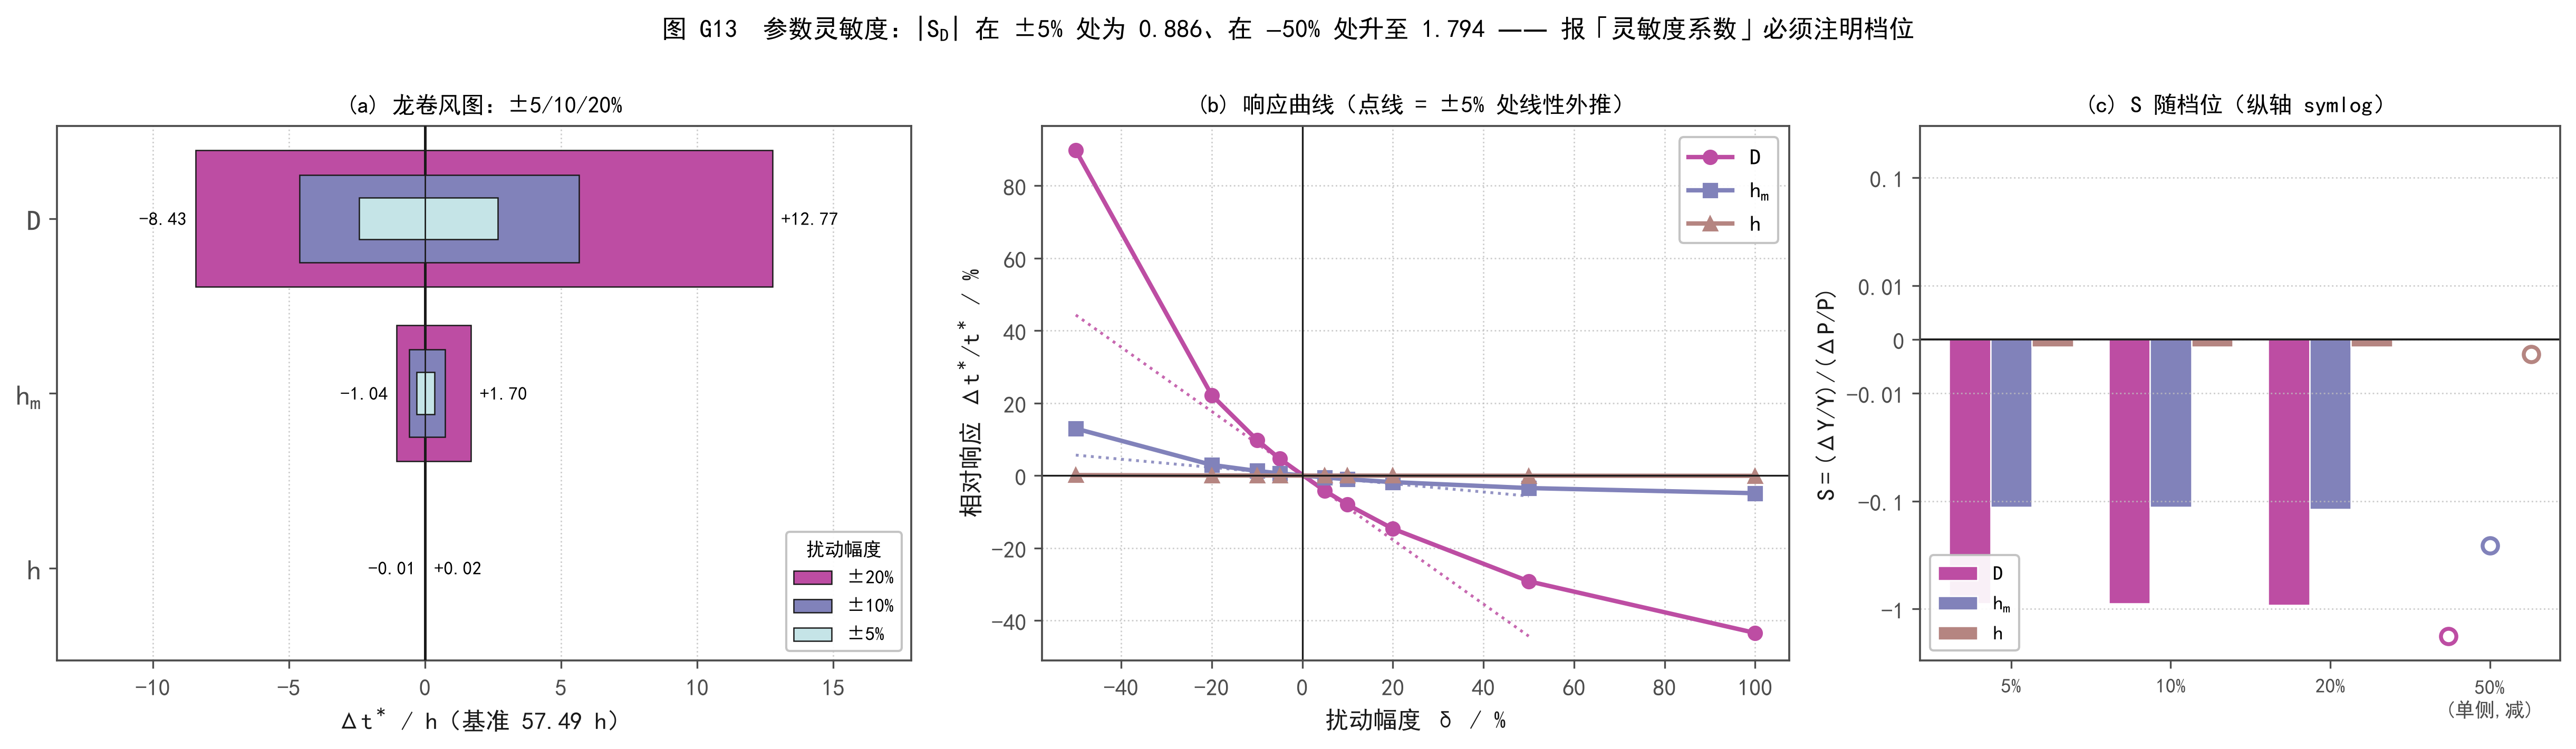
\includegraphics[width=\textwidth]{G13_tornado.png}
  \caption{参数灵敏度。(a) 龙卷风图（三档嵌套）；
           (b) 响应曲线与 $\pm5\%$ 处线性外推（点线）——
           实测在 $\lvert\delta\rvert\ge20\%$ 处系统性偏离线性；
           (c) 灵敏度系数随档位变化（纵轴 symlog）}
  \label{fig:G13}
\end{figure}

\subsubsection*{（2）与文献的对照}

\begin{table}[H]
  \centering
  \caption{灵敏度结论与文献的对照}
  \label{tab:lit}
  \footnotesize
  \begin{tabular}{@{}lll@{}}
    \toprule
    文献结论 & 本项目实测 & 判定 \\
    \midrule
    $S_D\approx0.65\sim0.78$（$D$ 最敏感）[R4-F21]
      & $S_D\approx-0.89$，排序第一且遥遥领先 & \textbf{证实}（量级同阶，本项目略高） \\
    $S_{h_m}<0.03$（$h_m$ 最不敏感）[R4-F21]
      & $S_{h_m}\approx-0.11$，是 $S_h$ 的 80 倍 & \textbf{证伪}（前提 $Bi_m\gg1$ 不成立） \\
    \bottomrule
  \end{tabular}
\end{table}

\subsubsection*{（3）三种区间分开命名}

\begin{table}[H]
  \centering
  \caption{三种区间严格分开}
  \label{tab:intervals}
  \footnotesize
  \begin{tabular}{@{}lll@{}}
    \toprule
    类型 & 本项目是否给出 & 值 \\
    \midrule
    \textbf{情景区间} & 给出
      & 参数倍率：$\tstar\in[32.53,109.06]$ h；环境外推：$[56.95,57.87]$ h \\
    \textbf{参数扰动分位区间} & 给出（仅 $D$ 一维）
      & 5\%$\sim$95\% 分位：$\tstar\in[43.48,77.21]$ h \\
    \textbf{数据扰动分位区间} & 给出（见 \S\ref{sec:robust}）
      & 见 表 \ref{tab:robust} \\
    \textbf{统计置信区间} & \textbf{不给} & 本工况没有批次测量数据 \\
    \bottomrule
  \end{tabular}
\end{table}

\begin{quote}
  三者\textbf{不得混称}，尤其\textbf{不得把情景区间说成置信区间}。
\end{quote}

\begin{figure}[H]
  \centering
  
\includegraphics[width=\textwidth]{G10_scenario.png}
  \caption{参数情景与区间}
  \label{fig:G10}
\end{figure}

% ==========================================================================
\subsection{稳健性检验：删数据 / 加噪声 / 换算法}
\label{sec:robust}

为检验结论对数据质量的依赖，本文对附件1 做三类扰动，每类独立重算
（共 63 次运行，基准 $57.488876$ h）：

\begin{table}[H]
  \centering
  \caption{数据扰动稳健性结果}
  \label{tab:robust}
  \footnotesize
  % C 行的三个数值串很长：原样排版时整表超出 \textwidth 55.9 pt（居中后左右各压出
  % 约 5 mm）。收紧列间距并去掉斜杠两侧的空格即可容下（实测），
  % 且**不增加行数** —— 这一点要紧：正文上限是 30 页，C 行一旦折行就会多出一页。
  \setlength{\tabcolsep}{2.5pt}
  \begin{tabular}{@{}llcccc@{}}
    \toprule
    扰动 & $n$ & 均值 $\tstar$ / h & $\sigma$ / s & 相对 & 极差 / s \\
    \midrule
    \textbf{A 随机删 10\%}（24/241 点） & 20 & 57.487533 & $\mathbf{30.0}$ & 0.015\% & 109.7 \\
    \textbf{B1 量化噪声}（附件末位精度） & 20 & 57.488872 & $\mathbf{0.22}$ & 0.0001\% & 0.8 \\
    \textbf{B2 传感器噪声}（假定 $\sigma_T$=0.1 $^\circ$C） & 20 & 57.483436 & $\mathbf{67.6}$ & 0.033\% & 192.6 \\
    \textbf{C 换插值算法} & 3 & PCHIP\,57.488876/SG\,57.489064/线性\,57.488871
      & --- & 差 $\mathbf{<0.7}$ s & --- \\
    \bottomrule
  \end{tabular}
\end{table}

三点结论：

\textbf{① 附件1 的记录精度不构成误差来源。}
量化噪声引起的散布为 $0.22$ s（$1\sigma$）/ $0.45$ s（$2\sigma$），
比时间离散误差（$1.86$ s）小 $4\sim8$ 倍，
比空间离散误差（$17.4$ s）小 $39\sim78$ 倍，\textbf{不可分辨}。
附件1 给到 $T$ 的 3 位小数是\textbf{够用的}。

\textbf{② 换插值算法不影响结论。} 三种算法给出的 $\tstar$ 相差不到 1 秒。

\textbf{③ ★ 数据扰动的影响经由``平台均值''单一渠道传递。}
对 20 个删除样本做回归，$\Delta\tstar/\Delta T_\infty=-1.850$ h/$^\circ$C，
\textbf{相关系数 $r=-0.9997$}；平台温度仅变动约 $0.016\ ^\circ$C
即决定了全部散布。\textbf{而长时平台取值本就是必须假定的量}——
其取法差异（4 档极差 $1090$ s）比本节全部数据扰动的总和（最大 $135$ s）
还大 \textbf{8 倍}。

\begin{figure}[H]
  \centering
  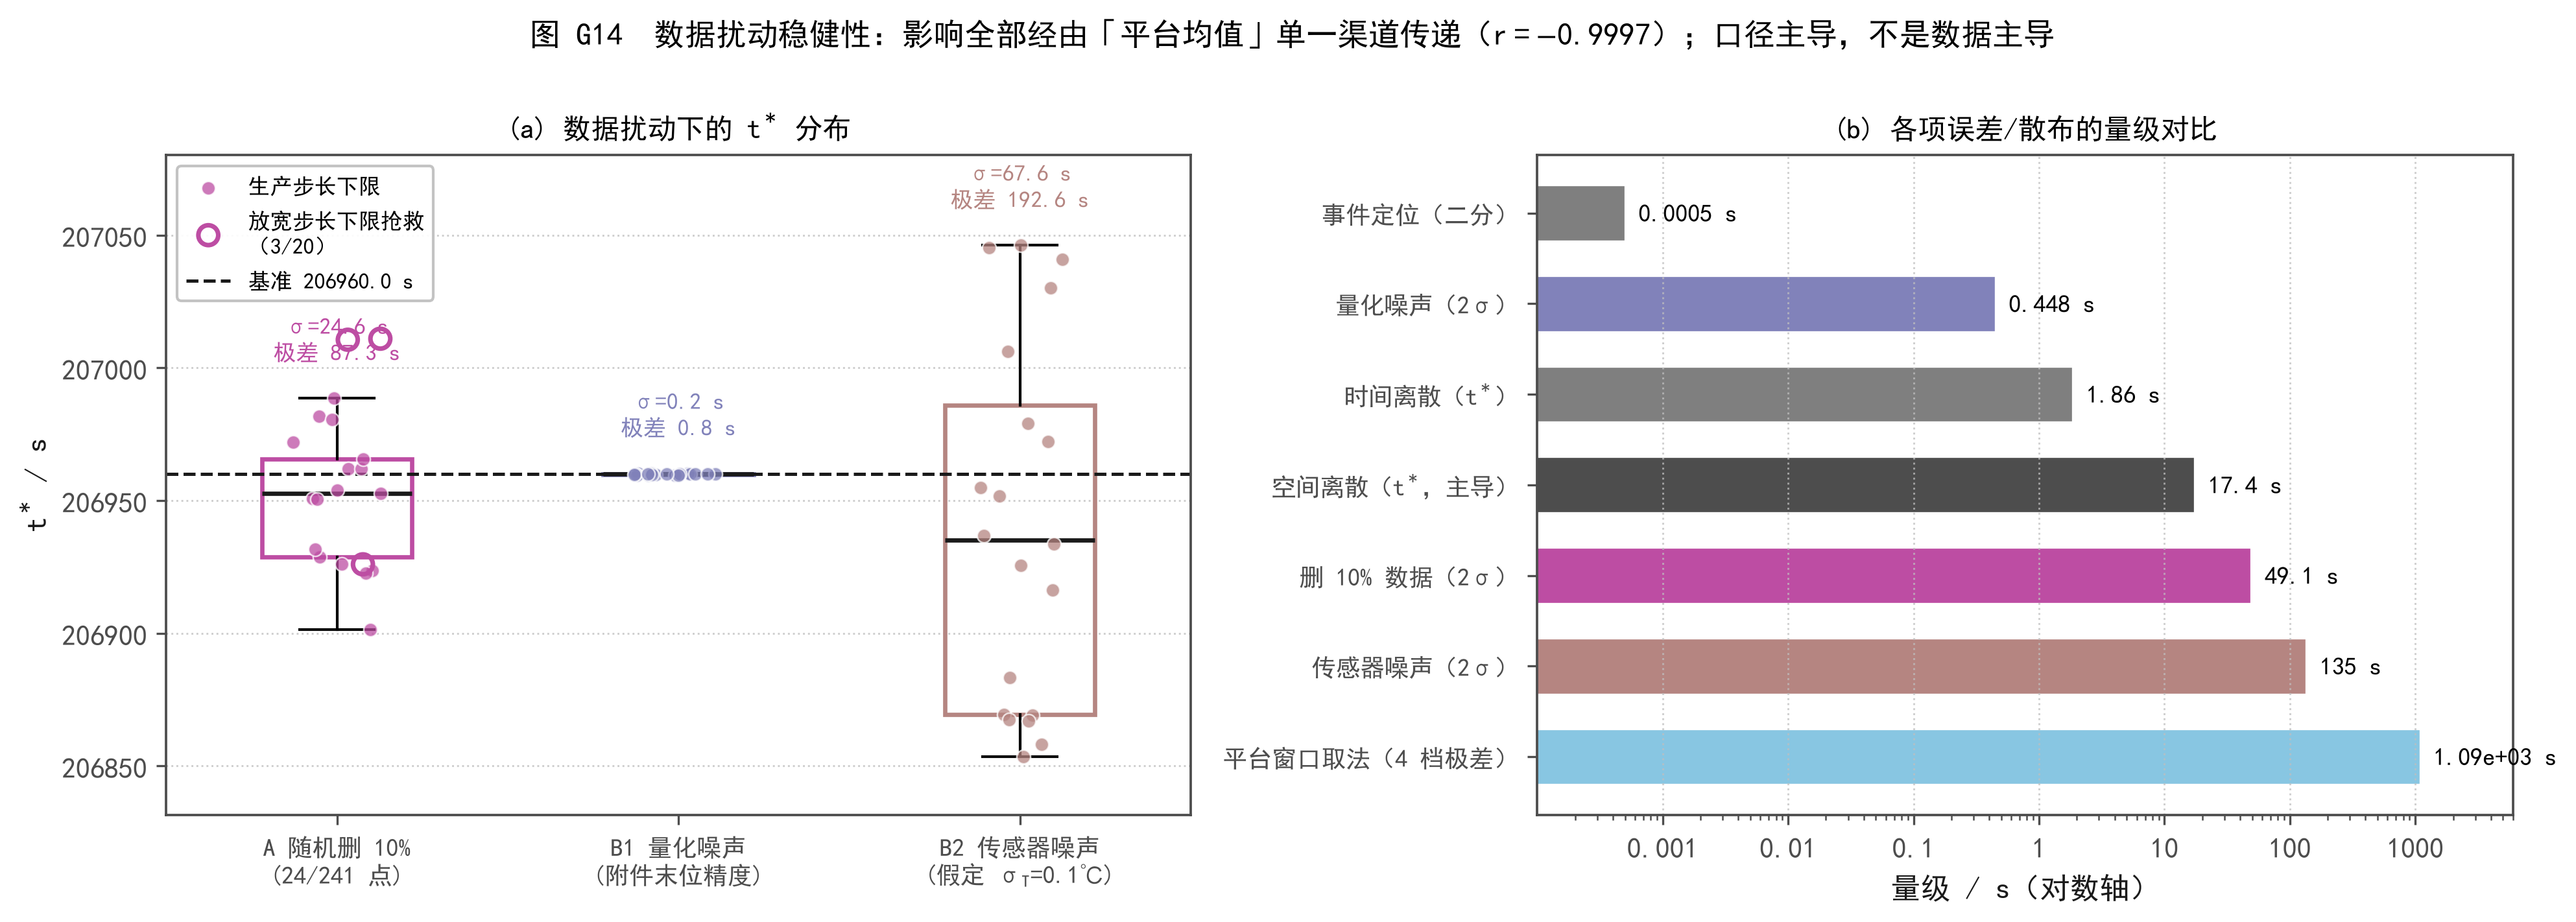
\includegraphics[width=\textwidth]{G14_robust.png}
  \caption{数据扰动稳健性。(a) 三组扰动下 $\tstar$ 的分布
           （空心圆为需放宽步长下限的 3 个删除样本）；
           (b) 各项误差与散布的量级对比——\textbf{平台窗口取法一项
           大于全部数据扰动之和}}
  \label{fig:G14}
\end{figure}

\begin{quote}
  \textbf{命名纪律（必须保留）}：上表三组扰动给出的散布为
  \textbf{「数据扰动分位区间」}，\textbf{不是统计置信区间}。
  附件1 是每 60 s 一条的\textbf{确定性采样时间表}，非随机样本；
  该散布刻画的是结果对\textbf{数据点集合}的敏感度，
  不含批次间真实变差（后者本文无数据）。\\
  \textbf{一处必须如实报告的异常}：20 个删除样本中有 3 个因删点后
  插值曲线局部变陡、触发生产步长下限（$\Delta t_{\min}=10^{-4}$ s）而无法求解；
  这 3 个样本改用放宽的 $\Delta t_{\min}=10^{-7}$ s 解出，
  其 $\tstar$ 均落在其余样本的分布范围内，
  $\sigma$ 从 $0.00683$ h 变为 $0.00834$ h（$+22\%$），\textbf{结论方向不变}。
\end{quote}

% ==========================================================================
\subsection{误差预算总表}
\label{sec:errbudget}

把本文所有已知的误差与散布项放在同一尺度上：

\begin{table}[H]
  \centering
  \caption{误差预算总表}
  \label{tab:budget}
  \footnotesize
  \begin{tabular}{@{}llc@{}}
    \toprule
    项 & 量级 / s & 来源 \\
    \midrule
    事件定位（二分收敛） & $0.0005$ & \S\ref{sec:tstar-err} \\
    B1 量化噪声（$2\sigma$） & $0.45$ & \S\ref{sec:robust} \\
    换插值算法（PCHIP/SG/线性） & $0.7$ & \S\ref{sec:robust} \\
    时间离散（$\tstar$） & $1.86$ & \S\ref{sec:tstar-err} \\
    \textbf{空间离散（$\tstar$，数值主导）} & $\mathbf{17.4}$ & \S\ref{sec:tstar-err} \\
    A 删 10\% 数据（$2\sigma$） & $60.0$ & \S\ref{sec:robust} \\
    B2 传感器噪声（$2\sigma$） & $135.2$ & \S\ref{sec:robust} \\
    \textbf{平台窗口取法（4 档极差）} & $\mathbf{1090}$ & \S\ref{sec:tstar-precision} \\
    \bottomrule
  \end{tabular}
\end{table}

\begin{quote}
  \textbf{本文的可信度瓶颈在建模约定，而非数据质量。}
  最大的两项是\textbf{长时环境平台的取法}（$1090$ s）与\textbf{空间离散}
  （$17.4$ s），而所有数据扰动加起来都超不过 $135$ s。
  这也正是本文把``精度口径声明''写进正文（\S\ref{sec:tstar-precision}）的原因。
\end{quote}

\section{模型改进与推广}

\subsection{蒸发潜热对照（M1，条件性扩展）}
\label{sec:M1}

问题2/3 的 M0 基线\textbf{不含蒸发潜热}。作为对照，M1 在表面能量平衡中加入潜热项
\begin{equation}
  -k\frac{\partial T}{\partial r}\bigg|_{R}=h\left(T_s-T_\infty\right)+\lambda J_w,
  \qquad
  J_w=\rho_d\,h_m\left(C_s-\Cinf\right),
\end{equation}
其中 $J_w$ 的单位是 kg/(m$^2\cdot$s)，\textbf{不得}把 $h_m(C_s-\Cinf)$
直接乘潜热当热通量——它的单位是 kg/(kg$\cdot$s)，不是 kg/(m$^2\cdot$s)，
必须乘密度基准 $\rho_d$。

\begin{table}[H]
  \centering
  \caption{M0 与 M1 的对照}
  \label{tab:M1}
  \footnotesize
  \begin{tabular}{@{}lccc@{}}
    \toprule
    项 & M0 & M1 & 差 \\
    \midrule
    3 h 中心温度 & $49.849\ ^\circ$C & $31.786\ ^\circ$C & $\mathbf{-18.06}$ K \\
    3 h 表面温度 & $49.967\ ^\circ$C & $32.402\ ^\circ$C & $-17.56$ K \\
    3 h 中心含水率 & 1.7662 & 2.2515 & $+0.485$（\textbf{更慢}） \\
    $\tstar$ & 57.49 h & 60.33 h & $\mathbf{+2.84}$ h（$\times1.049$） \\
    \bottomrule
  \end{tabular}
\end{table}

\begin{quote}
  \textbf{与文献的定量交叉验证}：文献 [1b] 报道``忽略潜热会使初期物料温度预测
  偏高 $12\sim22\ ^\circ\mathrm{C}$''。本项目独立复现的差值是 $\mathbf{18.06}$ K，
  \textbf{落在该区间内}——一次独立定量印证。
\end{quote}

\begin{figure}[H]
  \centering
  
\includegraphics[width=0.75\textwidth]{FIG-43_latent.png}
  \caption{潜热开关对照}
  \label{fig:FIG43}
\end{figure}

\textbf{为什么不能据此修订问题3 答案}：M1 的量级\textbf{正比于干基密度 $\rho_d$}，
而 $\rho_d$ 在本题中\textbf{没有给定}：

\begin{itemize}[leftmargin=1.6em, itemsep=2pt]
  \item 附录3 的 $\rho(C)=650+128C$ 是\textbf{湿物料体积密度}；
  \item 由它反推的 $\rho_d=\rho(C)/(1+C)$ 在 $C=0$ 给 650、在 $C=2.55$ 给 275.0
        ——\textbf{不是常数}，与``干物质守恒''\textbf{不兼容}；
  \item 本项目取\textbf{初始状态基准} $\rho_d=976.4/3.55=275.042$ kg/m$^3$
        并\textbf{显式声明}。
\end{itemize}

$\rho_d$ 翻倍则潜热效应翻倍（严格正比，相邻比 $2.03\sim2.07$）：

\begin{table}[H]
  \centering
  \footnotesize
  \begin{tabular}{@{}lccc@{}}
    \toprule
    $\rho_d$ 倍率 & $\rho_d$ / (kg/m$^3$) & $\tstar$ / h & $\Delta$ vs M0 \\
    \midrule
    0.25 & 68.76 & 58.17 & $+0.68$ h \\
    0.50 & 137.52 & 58.87 & $+1.38$ h \\
    \textbf{1.00（本文采用）} & \textbf{275.04} & \textbf{60.33} & $\mathbf{+2.84}$ h \\
    2.00 & 550.08 & 63.37 & $+5.88$ h \\
    \bottomrule
  \end{tabular}
\end{table}

\begin{quote}
  \textbf{结论}：M1 只能写成``\textbf{在本文声明的 $\rho_d$ 取值下}，
  蒸发潜热使 3 h 中心温度低约 18 K、使 $\tstar$ 延长约 2.8 h''。
  \textbf{不得}写成``药材真实烘干时间应为 60.3 h''，
  也\textbf{不得}用 M1 替换问题3 的答案。
\end{quote}

\subsection{烘房系统模型（M2 工程推广）}

本文把烘房环境作为\textbf{给定边界}（单向驱动），这是 M0 的合理简化。
若需预测新工况（改变装料量、换气量、加热策略），
应升级为\textbf{烘房—物料双向耦合系统模型}。正确的水分收支形式
（简化充分混合空气）为
\begin{equation}
  \frac{\mathrm d}{\mathrm dt}\left(M_{da}Y\right)
  =\dot m_{da,\mathrm{in}}Y_{\mathrm{in}}
   -\dot m_{da,\mathrm{out}}Y+\sum_i A_i J_{w,i}-\dot m_{\mathrm{cond}},
\end{equation}
还需\textbf{干空气质量平衡}。

\begin{quote}
  若 $M_{da}$ 不变，才可写成 $M_{da}\dot Y$；
  \textbf{不能用 $V_{air}\dot Y$ 等于质量流率的形式}——量纲不闭合。
\end{quote}

\textbf{数据需求}：空气干质量、装料量、加热与排湿条件、
新风/排风干空气质量流量或除湿速率。
\textbf{验证方式}：选择实测环境作为验证数据，
\textbf{不能同时将环境固定与自由求解}。

\subsection{品质后处理（M2 推广）}

有目标成分动力学后，可沿材料轨迹计算成分保留分数：
\begin{equation}
  \frac{q(t)}{q(0)}=\exp\left[-\int_0^t k_q\!\left(T(\tau),C(\tau)\right)\mathrm d\tau\right].
\end{equation}
这是\textbf{待标定的候选动力学}，不是文献为本题药材提供的通用公式。

\begin{table}[H]
  \centering
  \footnotesize
  \begin{tabular}{@{}ll@{}}
    \toprule
    扩展方向 & 额外数据需求 \\
    \midrule
    微生物 & 水活度关系 $a_w(C,T)$、菌种、初始菌量 \\
    结构（结壳 / 开裂） & 应变、本构关系、强度参数 \\
    挥发成分保留 & 成分种类、组织结构、动力学参数 \\
    \bottomrule
  \end{tabular}
\end{table}

\textbf{无水活度关系时}：只能说明``含水率达标 $\ne$ 微生物合格''，
\textbf{不能制定通用杀菌温度}。

\subsection{结构力学（M2 路线）}

建模链路（仅作路线描述）：
湿度场 $\to$ 收缩应变 $\to$ 本构关系 $\to$ 应力场 $\to$ 断裂判据 $\to$ 诊断量。

\begin{quote}
  不能由湿度梯度直接算裂纹概率或裂纹位置，
  也不能把``多缩 $7\%$''当作仿射收缩的验证。
  可输出梯度作为\textbf{非标定诊断量}，但不叫``裂纹概率''。
  \textbf{题目半径数据不证明内部均匀收缩。}
\end{quote}

\section{模型优缺点与取舍论证}

\subsection{优点与缺点}

本文方法的长处在于\textbf{离散格式与验证体系}：单向耦合洞察与双向耦合求解分开处理；
渐变网格 $N=200/\gamma=1.5$ 以约一半计算量取得优于均匀 $N=640$ 的精度；
L-稳定的 Backward Euler 规避显式稳定性上限 $0.37$ s；Picard 迭代保持 M-矩阵性质、
$C$ 的正性由构造保证；中心半控制体规避 $1/r$ 奇点，界面用调和平均
（$D$ 跨 7 个数量级时算术平均会高估通量）；入口检查 6 项明确 $C$ vs $Y$、
$\rho$ 定义、$T$ 单位与外推方式；五类检验齐备；材料坐标处理收缩时
$\dot R$ 对流项可证为零、两项 $R$ 幂次不可合并；A/B/C 顺序差分把物性与几何效应分开报告。

不足在于\textbf{数据与维度限制}：表面列在极早期欠分辨（$t=1$ s 处
$\Delta C=2.0\times10^{-4}$）；M0 不含蒸发潜热；一维轴对称简化，端面未做全面 CFD；
附件1 只覆盖 0--4 h，问题2/3 需外推；$\rho$ 为湿物料体积密度，
$\rho_d=\rho/(1+C)$ 与干物质守恒不兼容；时间收敛阶受参照解自身误差污染
（拟合 $+1.29\sim+1.43$），故只声称不低于一阶；$\rho_d$ 不确定，
$D$ 分位区间只传播 $D$ 一维；问题2 全程版按 60 s 采样；
缺少内部位移、水活度关系、目标成分动力学与应变/本构/强度参数；
3 个删数据样本需放宽步长下限才能解出（已如实报告，见 \S\ref{sec:robust}）。



\begin{enumerate}[leftmargin=2.2em, itemsep=2pt]
  \item \textbf{表面列在极早期欠分辨}：$t=1$ s 处 $\Delta C=2.0\times10^{-4}$；
  \item \textbf{M0 不含蒸发潜热}：表面温度系统性偏高；
  \item \textbf{一维轴对称简化}：端面方向尺度比 $39.06$，未做全面 CFD；
  \item \textbf{附件1 只覆盖 0--4 h}：问题2/3 需外推；
  \item \textbf{$\rho$ 为湿物料体积密度}：$\rho_d=\rho/(1+C)$
        与干物质守恒不兼容（见 \S\ref{sec:geo-density}）；
  \item \textbf{时间收敛阶的参照污染}：拟合 $+1.29\sim+1.43$（理论 $+1$）；
  \item \textbf{$\rho_d$ 不确定}：附录3 的 $\rho(C)/(1+C)$ 在 $275\sim650$ 间变化；
  \item \textbf{$D$ 分位区间只传播 $D$ 一维}：不是总不确定度；
  \item \textbf{问题2 全程版按 60 s 采样}：题面要求``每隔 1 s''；
  \item \textbf{未完成生产网格 vs 细参考网格的逐点对比}：参照网格超出机时预算；
  \item \textbf{缺少内部位移数据}：附件2 只给整体半径，
        无法识别内部位移是否仿射；
  \item \textbf{缺少水活度关系}：题目未给吸附等温线，无法做严格的气固转换；
  \item \textbf{缺少目标成分动力学、应变/本构/强度参数}；
  \item \textbf{3 个删数据样本需放宽步长下限}才能解出
        （见 \S\ref{sec:robust}，已如实报告）。
\end{enumerate}

\subsection{被省略因素的判据化取舍}
\label{sec:omitted}

本文识别出 \textbf{13 条}文献中提及、但未进入四问答案的因素。
\textbf{任何一条被排除，都归属且仅归属于三类判据之一}，
这一框架杜绝了``文献有但我没做''式的无判据省略：

\begin{table}[H]
  \centering
  \caption{三类判据（互斥且穷尽）}
  \label{tab:criteria}
  \footnotesize
  \begin{tabular}{@{}clc@{}}
    \toprule
    判据 & 含义 & 条数 \\
    \midrule
    \textbf{A 量级判据} & 该效应在本工况下小于判据所能分辨的尺度 & 3 \\
    \textbf{B 数据判据} & 题面\textbf{未给}该效应必需的参数，引入即等于编造参数 & 7 \\
    \textbf{C 重复计算判据} & 题给公式\textbf{已经隐含}了该效应 & 3 \\
    \bottomrule
  \end{tabular}
\end{table}

\begin{table}[H]
  \centering
  \caption{13 条因素的归属}
  \label{tab:13}
  \footnotesize
  \begin{tabularx}{\textwidth}{@{}clX@{}}
    \toprule
    判据 & 条数 & 因素 \\
    \midrule
    B 数据缺失 & 7
      & 蒸气渗流、辐射、结合水、干裂、各向异性、批次差异，
        以及 $\rho_d$ 的取值 \\
    A 量级/口径 & 3
      & Soret 效应（占费克通量 $0.3\sim1.1\%$）、
        控温波动（衰减 $>99\%$）、端面（最大值口径下 $<10^{-5}$） \\
    C 重复计算 & 3
      & 结壳、玻璃化（附录3 的 $e^{-0.45/C}$ \textbf{已含 16.8 倍衰减}）、
        双向耦合（\textbf{实测边界已含耦合}） \\
    \bottomrule
  \end{tabularx}
\end{table}

其中\textbf{因素``双向耦合''值得单独说明}：文献指出解耦会带来 $22\%\sim35\%$ 偏差，
但\textbf{本文直接采用附件1 实测的烘房温湿度}，
物料蒸发对烘房的反作用\textbf{已经在数据里}——
所以不是``忽略''，而是``自然消解''。

\textbf{三个已经建模并量化、但同样不进入答案的因素}，
其排除理由\textbf{各不相同}，必须分开写清楚：

\begin{table}[H]
  \centering
  \caption{三个已建模因素的处置与理由}
  \label{tab:3factors}
  \footnotesize
  \begin{tabularx}{\textwidth}{@{}lccX@{}}
    \toprule
    因素 & 进入答案 & 实测影响 & 为何这样处理 \\
    \midrule
    \textbf{蒸发潜热} & 否 & $\tstar$ $+2.84$ h（$+4.9\%$）
      & 题面未给 $\lambda$，且修正量正比于题面未定的 $\rho_d$ \\
    \textbf{端面效应} & 否 & 对 $\tstar$ $<10^{-5}$；
        对体积平均 $-2.2\%\sim-6.2\%$
      & 判据是全域最大值，端面影响不到几何中心 \\
    \textbf{结壳/玻璃化} & 否 & $\tstar$ $+42\%\sim+970\%$
      & 附录3 的 $D(C,T)$ 已含低含水率衰减，再乘会重复计算 \\
    \bottomrule
  \end{tabularx}
\end{table}

\section{结论}

本文建立一维轴对称径向热湿耦合模型，采用半控制体 FVM 与隐式时间推进求解，
回答了四个问题，并通过解析基准、收敛性、守恒、退化、灵敏度与稳健性六类检验验证模型。

\subsection{四问答案}

\begin{table}[H]
  \centering
  \caption{四个问题的答案}
  \label{tab:answers}
  \footnotesize
  \begin{tabularx}{\textwidth}{@{}clX@{}}
    \toprule
    问题 & 答案 & 关键说明 \\
    \midrule
    1 & 1800 s：中心 $33.58\ ^\circ$C、表面 $36.79\ ^\circ$C
      & 干燥只发生在表层（外侧约 0.7 cm）；中心含水率 30 min 内完全未变 \\
    2 & 3 h：中心 $49.85\ ^\circ$C、表面 $49.97\ ^\circ$C；
        中心 $1.77$、表面 $1.01$ kg/kg
      & 双向耦合使 1800 s 中心温度比问题1 低 $1.386\ ^\circ$C \\
    3 & $\tstar=\mathbf{57.49}$ h（$=206959.9521$ s $=2.40$ 天）
      & 判据必须是全域最大值；用面积平均会低估 $37.3\%$ \\
    4 & $\tdry=\mathbf{51.0906}$ h，终态半径 $1.2000$ cm
      & $\Delta t=1$ s 收敛口径；与另一套独立实现相差 $0.2\%$ \\
    \bottomrule
  \end{tabularx}
\end{table}

\subsection{检验结论与误差预算}

Bessel 解析基准误差 $<0.001\ ^\circ$C（相对 $<0.002\%$）；空间二阶
（实测 $+2.20$）、时间不低于一阶（\textbf{不声称二阶}）；
内部界面通量抵消达机器精度 $1.782\times10^{-16}$；五项退化与一致性检验通过；
跨实现逐行移植复现差 $+11$ s（$0.004\%$）。
几何—密度一致性诊断提示密度定义、数据误差、几何假设或干物质守恒的
联合使用需核查（\textbf{条件性结论，不下``数据有误''的判断}）。

误差预算（\S\ref{sec:errbudget}）的落点是\textbf{口径主导，不是数据主导}：
\textbf{平台窗口取法一项即达 $1090$ s，比最大的数据扰动（$135$ s）还大 8 倍}，
也远大于全部数值离散误差（约 $19$ s）。

\subsection{灵敏度与稳健性}

敏感度排序 $D\gg h_m\gg h$ 在五档扰动下均不变；
但 $|S_D|$ 在 $\pm5\%$ 处为 $0.886$、在 $-50\%$ 处为 $1.794$——
\textbf{灵敏度系数是局部量，报告时必须注明档位}。
数据扰动引起的散布为 $0.22\sim67.6$ s，\textbf{全部经由``长时平台均值''
单一渠道传递}（$r=-0.9997$）。
三种区间（情景 / 参数扰动分位 / 数据扰动分位）严格分开命名，
\textbf{统计置信区间不给}。

\subsection{模型局限与推广}

\textbf{局限}：一维轴对称简化，端面效应以二维对照验证而非全面 CFD；
M0 不含蒸发潜热（M1 对照显示 3 h 中心温度低 $18.06$ K、$\tstar$ 延长
$2.84$ h，属\textbf{条件性扩展，不改答案}）；附件1 只覆盖 0--4 h 需外推；
缺少内部位移、水活度、目标成分动力学等数据。

\textbf{推广}：烘房—物料双向耦合系统模型（需空气干质量、装料量、
新风/排风质量流量）；品质后处理（需水活度关系、成分动力学、菌种与初始菌量）；
结构力学（需应变、本构、强度参数）。


% ==================== AI 工具使用声明（必须在参考文献之前）====================
% 依据《全国大学生数学建模竞赛人工智能工具使用规定》第 3 条
% 依据《全国大学生数学建模竞赛人工智能工具使用规定》（2026 年试行）第 3 条：
% 「参赛队应在论文**参考文献之前**设置"AI 工具使用声明"，二者择一。」
% 本文属于「使用了 AI 工具」的情形，采用第（2）种声明。
% 详细使用情况另见支撑材料中的《AI 工具使用详情.pdf》（第 4 条要求）。

\section*{AI 工具使用声明}
\addcontentsline{toc}{section}{AI 工具使用声明}

本参赛队在竞赛过程中使用了 AI 工具，主要用于\textbf{代码调试与数值结果核验、
文献检索与出处核实、以及语言润色}，详细使用情况见支撑材料
《AI 工具使用详情.pdf》。

\vspace{2pt}
\noindent\textbf{核心建模与分析的自主性声明}：

\begin{enumerate}[leftmargin=2.2em, itemsep=2pt]
  \item 本文的\textbf{物理模型、控制方程、边界条件、数值格式与判据口径}
        均由参赛队自主确定；AI 工具不参与模型选择与建模决策。
  \item 本文\textbf{全部数值结果}由参赛队编写的求解程序计算产生。
        AI 工具用于代码调试与结果核验，其输出\textbf{逐项经过人工审查}：
        凡由 AI 辅助发现的代码缺陷，均要求提供\textbf{可复现的最小反例}后
        才予采纳（例如"误差随步长收敛阶被 $\log 0$ 污染而虚高"、
        "台账合并误删历史记录"两处，都是先复现再修）。
  \item 本文\textbf{所有引用的数据与结论均可溯源}：
        题面与附件数据标【题面/附件】，文献结论标明出处与 DOI，
        本文自算量显式标注"本文计算得到"。
        \textbf{凡无法核实的外部数字一律不采用}（见 \S\ref{sec:refnote}）。
  \item AI 工具生成的文字\textbf{均经人工改写与核验}，
        并由参赛队对全文的数值一致性做了\textbf{自动校验}
        （逐条比对论文中的关键数值与结果文件，共 25 项）。
\end{enumerate}


% ==================== 参考文献 ====================
\begin{thebibliography}{99}
\addcontentsline{toc}{section}{参考文献}
\small

\bibitem{Q1} 2026 年高教社杯全国大学生数学建模竞赛 A 题《药材的烘干问题》题面
（含附录 1--4）.

\bibitem{Q2} 附件1：烘房温度与水分浓度（0--14400 s，241 点）.

\bibitem{Q3} 附件2：药材半径随时间的变化（0--259200 s，145 点）.

\bibitem{Q4} 附件3：result1--result4 结果模板.

\bibitem{kumar} Kumar, C., Millar, G. J., \& Karim, M. A. (2015).
\emph{Effective diffusivity and evaporative cooling in convective drying of
food material.} Drying Technology, \textbf{33}(2), 227--237.
DOI: \texttt{10.1080/07373937.2014.947512}.

\bibitem{defraeye} Defraeye, T., Blocken, B., \& Carmeliet, J. (2012).
\emph{Analysis of convective heat and mass transfer coefficients for convective
drying of a porous flat plate.} International Journal of Heat and Mass Transfer,
\textbf{55}(1--3), 36--48.
DOI: \texttt{10.1016/j.ijheatmasstransfer.2011.08.047}.

\bibitem{datta} Datta, A. K. (2007).
\emph{Porous media approaches to studying simultaneous heat and mass transfer in
food processes. I: Problem formulations.} Journal of Food Engineering,
\textbf{80}(1), 80--95. DOI: \texttt{10.1016/j.jfoodeng.2006.05.013}.

\bibitem{vu} Vu, H. T., \& Tsotsas, E. (2018).
\emph{Mass and heat transport models for analysis of the drying process in
porous media: A review and numerical implementation.}
International Journal of Chemical Engineering, \textbf{2018}, 9456418.
DOI: \texttt{10.1155/2018/9456418}.

\bibitem{soret} H\"aussling L\"owgren, B., Bergmann, J., \& Alves-Filho, O. (2020).
\emph{A numerical implementation of the Soret effect in drying processes.}
ChemEngineering, \textbf{4}(1), 13.
DOI: \texttt{10.3390/chemengineering4010013}.

\bibitem{younsi} Younsi, R., Kocaefe, D., Poncs\'ak, S., \& Kocaefe, Y. (2007).
\emph{Comparison of different models for the high-temperature heat-treatment of
wood.} International Journal of Thermal Sciences, \textbf{46}(7), 707--716.
DOI: \texttt{10.1016/j.ijthermalsci.2006.09.001}.

\bibitem{gulati15} Gulati, T., \& Datta, A. K. (2015).
\emph{Mechanistic understanding of case-hardening and texture development during
drying of food materials.} Journal of Food Engineering, \textbf{166}, 119--138.
DOI: \texttt{10.1016/j.jfoodeng.2015.05.031}.

\bibitem{gulati12} Gulati, T., \& Datta, A. K. (2012).
\emph{Multiphase transport with large deformations undergoing rubbery-glassy
phase transition: Applications to drying.}
Proceedings of the 2012 COMSOL Conference, Boston.

\bibitem{khalloufi} Khalloufi, S., \& Bongers, P. (2012).
\emph{Mathematical investigation of the case hardening phenomenon explained by
shrinkage and collapse mechanisms occurring during drying processes.}
Computer Aided Chemical Engineering, \textbf{30}, 1068--1072.
DOI: \texttt{10.1016/B978-0-444-59520-1.50072-5}.

\bibitem{khan} Khan, M. I. H., Wellard, R. M., Nagy, S. A., et al. (2016).
\emph{Investigation of bound and free water in plant-based food material using
NMR $T_2$ relaxometry.}
Innovative Food Science \& Emerging Technologies, \textbf{38}, 252--261.
DOI: \texttt{10.1016/j.ifset.2016.10.015}.

\bibitem{sami} Sami, S., Rahimi, A., \& Etesami, N. (2011).
\emph{Dynamic modeling and a parametric study of an indirect solar cabinet
dryer.} Drying Technology, \textbf{29}(7), 825--835.
DOI: \texttt{10.1080/07373937.2010.545159}.

\bibitem{ceylan} Ceylan, \.I., Akta\c{s}, M., \& Do\u{g}an, H. (2007).
\emph{Mathematical modeling of drying characteristics of tropical fruits.}
Applied Thermal Engineering, \textbf{27}(11--12), 1931--1936.
DOI: \texttt{10.1016/j.applthermaleng.2006.12.020}.

\bibitem{takhar} Takhar, P. S., Maier, D. E., \& Campanella, O. H. (2011).
\emph{Hybrid mixture theory based moisture transport and stress development in
corn kernels during drying: Coupled model and validation.}
Journal of Food Engineering, \textbf{106}(2), 148--156.
DOI: \texttt{10.1016/j.jfoodeng.2011.05.006}.

\bibitem{curcio} Curcio, S., \& Aversa, M. (2014).
\emph{Influence of shrinkage on convective drying of fresh vegetables:
A theoretical model.} Journal of Food Engineering, \textbf{123}, 36--49.
DOI: \texttt{10.1016/j.jfoodeng.2013.09.014}.

\bibitem{pacheco} Pacheco-Aguirre, F. M., Ladr\'on-Gonz\'alez, A.,
Ru\'iz-Espinosa, H., et al. (2014).
\emph{A method to estimate anisotropic diffusion coefficients for cylindrical
solids: Application to the drying of carrot.}
Journal of Food Engineering, \textbf{125}, 24--33.
DOI: \texttt{10.1016/j.jfoodeng.2013.10.015}.

\bibitem{abbasi} Abbasi Souraki, B., \& Mowla, D. (2008).
\emph{Axial and radial moisture diffusivity in cylindrical fresh green beans in
a fluidized bed dryer with energy carrier: Modeling with and without shrinkage.}
Journal of Food Engineering, \textbf{88}(1), 9--19.
DOI: \texttt{10.1016/j.jfoodeng.2007.05.013}.

\bibitem{mercier} Mercier, S., Moresoli, C., Villeneuve, S., et al. (2013).
\emph{Sensitivity analysis of parameters affecting the drying behaviour of
durum wheat pasta.} Journal of Food Engineering, \textbf{119}(1), 1--11.
DOI: \texttt{10.1016/j.jfoodeng.2013.03.024}.

\bibitem{mortier} Mortier, S. T. F. C., Gernaey, K. V., De Beer, T., \&
Nopens, I. (2014).
\emph{Global sensitivity analysis applied to drying models for one or a
population of granules.} AIChE Journal, \textbf{60}(5), 1700--1717.
DOI: \texttt{10.1002/aic.14383}.

\bibitem{bhandari} Bhandari, B. R., \& Howes, T. (1999).
\emph{Implication of glass transition for the drying and stability of dried
foods.} Journal of Food Engineering, \textbf{40}(1--2), 71--79.
DOI: \texttt{10.1016/S0260-8774(99)00039-4}.

\bibitem{rahman} Rahman, M. S. (2006).
\emph{State diagram of foods: Its potential use in food processing and product
stability.} Trends in Food Science \& Technology, \textbf{17}(3), 129--141.
DOI: \texttt{10.1016/j.tifs.2005.09.009}.

\bibitem{champion} Champion, D., Le Meste, M., \& Simatos, D. (2000).
\emph{Towards an improved understanding of glass transition and relaxations in
foods: Molecular mobility in the glass transition range.}
Trends in Food Science \& Technology, \textbf{11}(2), 41--55.
DOI: \texttt{10.1016/S0924-2244(00)00047-9}.

\end{thebibliography}

\vspace{8pt}
\label{sec:refnote}


% ==================== 附录（页数不限）====================
\appendix

% 规范第五条：附录内容应包括**支撑材料的文件列表**。
% 规范第十一条：完整可运行的源程序随**支撑材料**提交。
% 为便于纸质打印与审阅，附录 B 不重复排印源码（原为 16 个模块全文，约 70 页），
% 改为**核心算法伪代码 + 源码索引**；伪代码与源码逐句对应。

% 🔴 修正：原先写成 \section{附录 A：…}，而 \appendix 已使 \thesection = A，
%    渲染结果重复成「A 附录 A：支撑材料文件列表」。现只写标题正文。
%    同时给附录内的表独立编号（表 A.1、B.1 …），避免与正文连续编号混排
%    （修正前附录第一张表编号为「表 38」）。
\setcounter{table}{0}
\renewcommand{\thetable}{\thesection.\arabic{table}}

% ==========================================================================
\section{支撑材料文件列表}
\setcounter{table}{0}

\noindent 支撑材料打包为单个压缩文件（\texttt{ZIP}，$<20$\,MB）。
\textbf{建模所用的全部完整、可运行源程序随支撑材料提交}，
其源码索引与核心算法伪代码见附录 B。目录结构与文件列表如下。

\begin{table}[H]
  \centering
  \caption{支撑材料目录结构}
  \label{tab:supportfiles}
  \footnotesize
  \begin{tabularx}{\textwidth}{@{}lX@{}}
    \toprule
    目录 / 文件 & 内容 \\
    \midrule
    \texttt{01\_result/} &
      四个正式结果 \texttt{result1--result4.xlsx}；
      各结果对应的 \texttt{resultN\_运行信息.xlsx}（网格、步长、口径与终止条件）；
      题设表 1--6；\texttt{说明.md} \\
    \texttt{02\_代码/00\_公共内核/} &
      完整 \texttt{src/} 包（\texttt{config}、\texttt{numerics}、\texttt{models}、
      \texttt{io}、\texttt{data\_prep}、\texttt{validation}、\texttt{figures}），
      保持 import 结构，\textbf{可直接运行} \\
    \texttt{02\_代码/01\_问题1/}\,$\cdots$\,\texttt{04\_问题4/} &
      各题专属模块与运行、校验脚本（四题共 24 个脚本），按题归档便于查阅 \\
    \texttt{02\_代码/README\_代码说明.md} &
      运行方法与全部脚本清单 \\
    \texttt{03\_参考文献/} &
      引用核实清单（含 DOI 反查结果）、原文 PDF、下载记录、文献研报与检索工具 \\
    \texttt{04\_提示词与分工清单/} &
      分工方案、论文骨架、被省略因素汇总、求解框架、论文修订记录 \\
    \texttt{05\_图片/} &
      全部 23 张插图的 PNG（300\,dpi）与 PDF（矢量）、出图脚本、图目录 \\
    \texttt{AI 工具使用详情.pdf} &
      依《人工智能工具使用规定》第 4 条提供 \\
    \texttt{README.md} & 支撑材料总说明与复现步骤 \\
    \bottomrule
  \end{tabularx}
\end{table}

\subsection*{A.1 运行环境}

Python 3.14.2、NumPy 2.4.4、SciPy 1.18.0、Matplotlib 3.11.0；
问题4 的对照实现另用 MATLAB。全部脚本纯 CPU、单线程即可复现；
除数据扰动 Monte Carlo 部分外不含随机数，该部分固定随机种子。

\subsection*{A.2 复现命令}

以 \texttt{02\_代码/00\_公共内核/} 为工作目录：

\begin{lstlisting}[language=bash, numbers=none]
pip install -r requirements.txt
python scripts/run_day3.py --stage all         # 问题1-3：冻结、收敛、复现
python scripts/run_p4.py   --stage all         # 问题4：主结果、网格、时间收敛
python scripts/p4_paper.py --stage all         # 论文口径的表6 与 B 方案
python scripts/run_sens_param.py --stage all   # 参数灵敏度 ±5/10/20%
python scripts/run_robust_data.py --stage all  # 数据扰动稳健性
\end{lstlisting}

% ==========================================================================
\section{核心算法伪代码与源码索引}
\setcounter{table}{0}

\noindent 建模与求解所用的\textbf{完整、可运行源程序}随支撑材料提交，
见附录 A 的 \texttt{02\_代码/}（\texttt{src/} 包共 30 个功能模块、另有 7 个包
\texttt{\_\_init\_\_} 文件；按题归档的运行与校验脚本 24 个）。
为便于纸质打印与复核，本附录\textbf{不重复排印源码}，
只给出核心算法的伪代码与源码索引（表 \ref{tab:srcindex} 的 16 个文件即求解内核
与两个主运行脚本，共 4192 行）。

\noindent 下列伪代码与源码\textbf{逐句对应}：每条算法下方标注其在支撑材料中的
文件与入口函数，行号与变量名均取自源码。

\subsection*{B.1 源码索引}

\begin{table}[H]
  \centering
  \caption{核心源码索引（路径前缀 \texttt{02\_代码/00\_公共内核/src/}）}
  \label{tab:srcindex}
  \footnotesize
  \begin{tabularx}{\textwidth}{@{}llrX@{}}
    \toprule
    模块 & 功能 & 行数 & 对应算法 \\
    \midrule
    \texttt{config.py}          & 配置与单位约定            & 196 & --- \\
    \texttt{numerics/properties.py} & 物性公式（附录2/3/4）& 158 & --- \\
    \texttt{numerics/fvm\_cyl.py}   & 有限体积离散内核     & 376 & 算法 \ref{alg:fvm} \\
    \texttt{numerics/nonlinear.py}  & Picard 迭代与双重判据 & 110 & 算法 \ref{alg:fvm}\,/\,\ref{alg:picard} \\
    \texttt{numerics/time\_stepper.py} & Backward Euler 自适应步长 & 293 & 算法 \ref{alg:stepper} \\
    \texttt{numerics/coupled.py}    & 双向耦合块迭代       & 179 & 算法 \ref{alg:picard} \\
    \texttt{models/boundary.py}     & 边界条件（M0 + M1 潜热） & 271 & 算法 \ref{alg:fvm} \\
    \texttt{data\_prep/env\_interp.py}  & 环境插值（附件1） & 159 & --- \\
    \texttt{data\_prep/env\_extrap.py}  & 长时环境外推（平台值） & 155 & --- \\
    \texttt{models/problem1.py}     & 问题1 求解           & 146 & --- \\
    \texttt{models/problem2.py}     & 问题2 求解（全程变物性） & 340 & --- \\
    \texttt{models/problem3.py}     & 问题3 阈值通过时刻   & 248 & 算法 \ref{alg:threshold} \\
    \texttt{models/problem4.py}     & 问题4 材料坐标与收缩 & 292 & 算法 \ref{alg:material} \\
    \texttt{models/problem3\_2d.py} & 问题3 二维轴对称端面对照 & 392 & --- \\
    \texttt{scripts/run\_day3.py}   & 主运行脚本（问题1--3，写盘 result1--3） & 621 & --- \\
    \texttt{scripts/run\_p4.py}     & 主运行脚本（问题4，写盘 result4） & 256 & --- \\
    \midrule
    合计 & 16 个文件 & \textbf{4192} & 5 个算法 \\
    \bottomrule
  \end{tabularx}
\end{table}

\noindent 表中\textbf{行数由脚本统计}，等于各文件实际行数之和。
未列入本表的还有 \texttt{validation/}（解析基准、守恒量、收敛阶等 5 个校验模块）、
\texttt{figures/}（出图）、\texttt{io/}（写盘与重采样）等辅助模块，
以及按题归档的 24 个运行与校验脚本（参数灵敏度、数据扰动、端面对照等），
一并随支撑材料提交。

% ---------------------------------------------------------------- 算法 1
\subsection*{B.2 算法 \ref{alg:fvm}：圆柱半控制体有限体积装配}

\begin{algorithm}[H]
\caption{圆柱半控制体有限体积装配（\texttt{fvm\_cyl.py}：\texttt{assemble}，第 195--282 行）}
\label{alg:fvm}
\Input{单元扩散系数 $\Gamma_i$（传热取 $k$，传质取 $D$）；表面对流系数 $h$；
       环境值 $\phi_\infty$；网格 $\{r_f,r_c,h,V,A\}$；
       体积热容 $\mathrm{cap}_i$（仅变物性传热用，否则为 \texttt{None}）}
\Output{三对角算子 $(\mathbf d,\boldsymbol\ell,\mathbf u,\mathbf b)$ 与 $\mathrm{Bi}_\Delta$，
        使 $\dot\phi = M\phi+\mathbf b$}
\BlankLine
$\Gamma_f \gets$ 面扩散系数
  \Comment*[r]{调和平均 $\Gamma_f[j]=\frac{2\Gamma_{j-1}\Gamma_j}{\Gamma_{j-1}+\Gamma_j}$，端点取单侧值}
$V^d_i \gets V_i\cdot\mathrm{cap}_i$
  \Comment*[r]{守恒形式整体除以 $(\rho c_p)_iV_i$；\texttt{None} 时 $V^d_i\gets V_i$}
\BlankLine
\Comment*[r]{中心控制体 $i=0$：$r=0$ 面通量恒为 0，半圆柱体积天然规避 $1/r$ 奇点}
$c_0 \gets A_1\Gamma_f[1]/(h_0V^d_0)$\;
$d_0 \gets -c_0$，$u_0 \gets +c_0$\;
\BlankLine
\For{$i \gets 1$ \KwTo $N-2$}{
  \Comment*[r]{内部单元：内、外两个面各贡献一项}
  $a^- \gets A_i\Gamma_f[i]/(h_{i-1}V^d_i)$\;
  $a^+ \gets A_{i+1}\Gamma_f[i+1]/(h_iV^d_i)$\;
  $d_i \gets -(a^-+a^+)$，$\ell_i \gets a^-$，$u_i \gets a^+$\;
}
\BlankLine
\Comment*[r]{表面单元 $i=N-1$：Robin 条件 $\partial\phi/\partial r\approx(\phi_s-\phi_N)/d$ 与}
\Comment*[r]{线性剖面联立，消去面值 $\phi_s$（单元中心格式的二阶边界处理）}
$d \gets R_0-r_c[N-1]$\;
\eIf{$\Gamma_f[N]>0$ 且 $d>0$}{
  $\mathrm{Bi}_\Delta \gets h\,d/\Gamma_f[N]$\;
  $\beta \gets A_N h/\bigl[(1+\mathrm{Bi}_\Delta)V^d_{N-1}\bigr]$\;
}{
  $\mathrm{Bi}_\Delta \gets \infty$，$\beta \gets A_N h/V^d_{N-1}$\;
}
$a^+ \gets A_{N-1}\Gamma_f[N-1]/(h_{N-2}V^d_{N-1})$\;
$d_{N-1} \gets -(a^++\beta)$，$\ell_{N-1} \gets a^+$，$b_{N-1} \gets \beta\phi_\infty$\;
\Return $(\mathbf d,\boldsymbol\ell,\mathbf u,\mathbf b)$，$\mathrm{Bi}_\Delta$\;
\end{algorithm}

\noindent\textbf{说明}：传热时 $\Gamma_i$ 传 $k$（W/(m$\cdot$K)）、$h$ 传
\textbf{未归一化的} $h$（W/(m$^2\cdot$K)），由 $\mathrm{cap}_i=(\rho c_p)_i$ 完成归一化；
传质时 $\Gamma_i$ 传 $D$、$h$ 传 $h_m$，二者量纲同为 m/s。
\textbf{$k$ 在面上取调和平均、$(\rho c_p)$ 在单元上取值，两者不可合并} ——
若误令 $\Gamma=k/(\rho c_p)$ 再走同一条路径，等于把 $k$ 与 $\rho c_p$
在同一个面上一起做调和平均，与本工况 $\rho c_p$ 沿 $r$ 变化数倍的事实不符。

% ---------------------------------------------------------------- 算法 2
\subsection*{B.3 算法 \ref{alg:picard}：双向耦合的块 Gauss--Seidel Picard 迭代}

\begin{algorithm}[H]
\caption{双向耦合块迭代（\texttt{coupled.py}：\texttt{block\_picard\_solve}，第 71--154 行）}
\label{alg:picard}
\Input{上一时刻解 $T^n,C^n$；步长 $\Delta t$ 与 $\theta$；
       两个装配回调 $\mathrm{assemble}_C(C,T)$、$\mathrm{assemble}_T(T,C)$；
       收敛容差 \texttt{tol\_T}/\texttt{tol\_C}}
\Output{$T^{n+1},C^{n+1}$ 及迭代记录（迭代数、更新量、真残差）}
\BlankLine
$T \gets T^n$，$C \gets C^n$，$\mathrm{prev} \gets \infty$\;
\For{$k \gets 1$ \KwTo \texttt{max\_iter}}{
  \Comment*[r]{① 水分场：$D=D(C,T)$ 显含温度，故须用当前 $T$}
  $M_C \gets \mathrm{assemble}_C(C,T)$\;
  $C \gets$ 隐式单步$(M_C, C^n, \Delta t, \theta)$\;
  \BlankLine
  \Comment*[r]{② 温度场：用\textbf{最新}的 $C$（Gauss--Seidel，非 Jacobi）}
  $M_T \gets \mathrm{assemble}_T(T,C)$\;
  $T \gets$ 隐式单步$(M_T, T^n, \Delta t, \theta)$\;
  \BlankLine
  \Comment*[r]{③ 双重判据：更新量\textbf{与}真残差都必须满足}
  $\mathrm{upd} \gets \max\bigl(\mathrm{upd}_T,\mathrm{upd}_C\bigr)$，
  $\mathrm{upd}_\bullet = \max_i\dfrac{|u^{k+1}_i-u^k_i|}{\mathrm{atol}_u+\mathrm{rtol}_u|u^{k+1}_i|}$\;
  \Comment*[r]{真残差：在\textbf{新解处重新装配}算子后计算 $F(u^{k+1})$}
  $F \gets (u-u^n)/\Delta t - M(u)\,u - \mathbf b(u)$\;
  $\mathrm{res} \gets \max\bigl(\mathrm{res}_T,\mathrm{res}_C\bigr)$，
  $\mathrm{res}_\bullet = \max_i\dfrac{|F_i|}{\mathrm{atol}_r+\mathrm{rtol}_r\max(|u_i/\Delta t|,10^{-3})}$\;
  \BlankLine
  \If{$\mathrm{upd}\le 1$ \textbf{且} $\mathrm{res}\le 1$}{
    \Return $T,C$，\texttt{converged}$\gets$真\;
  }
  \Comment*[r]{停滞检测：更新量不再显著下降即失败，交由外层折半步长重试}
  \If{$k>3$ \textbf{且} $\mathrm{upd}>0.5\,\mathrm{prev}$ \textbf{且} $\mathrm{upd}>1$}{
    \textbf{抛出} \texttt{NonlinearFailure}\;
  }
  $\mathrm{prev} \gets \mathrm{upd}$\;
}
\textbf{抛出} \texttt{NonlinearFailure}（达到最大迭代次数）\;
\end{algorithm}

\noindent\textbf{为什么用 Picard 而非 Newton}：每次子求解的迭代矩阵保持
\textbf{M-矩阵}性质，离散极值原理成立，$C$ 与 $T$ 的正性由构造保证，
无需任何裁剪，也不会像 Newton 那样过冲进入 $\exp(-0.89/C)$ 的悬崖区。
\textbf{为什么残差判据不可省}：只检查更新量会落入``更新量变小但残差停滞''
的陷阱；本工况在 $\Delta t$ 较大时曾实际出现。

% ---------------------------------------------------------------- 算法 3
\subsection*{B.4 算法 \ref{alg:stepper}：隐式自适应时间推进与事件早停}

\begin{algorithm}[H]
\caption{自适应时间推进（\texttt{time\_stepper.py}：\texttt{AdaptiveStepper.integrate}，第 107--287 行）}
\label{alg:stepper}
\Input{初值 $(t_0,u_0)$；终止时刻 $t_{\text{end}}$；输出时刻表 $t_{\text{out}}$；
       单步回调 $\Phi$；事件函数 \texttt{stop\_fn}；容差 $\mathrm{atol},\mathrm{rtol}$}
\Output{输出时刻上的解序列 $u_k$、步长历史、终止原因}
\BlankLine
$t \gets t_0$，$u \gets u_0$，$\Delta t \gets \Delta t_0$\;
\While{$t < t_{\text{end}}$}{
  $\Delta t \gets \min\bigl(\Delta t,\ t_{\text{out,next}}-t\bigr)$
    \Comment*[r]{裁剪到恰好落在下一个输出时刻 —— \textbf{输出从不靠插值}}
  \BlankLine
  \Comment*[r]{Richardson 误差估计：一步全步长 与 两步半步长 之差}
  $u_{\text{full}} \gets \Phi(t,u,\Delta t)$\;
  $u_{\text{half}} \gets \Phi\bigl(t+\tfrac{\Delta t}{2},\Phi(t,u,\tfrac{\Delta t}{2}),\tfrac{\Delta t}{2}\bigr)$\;
  $\mathrm{err} \gets \max_i\dfrac{|u_{\text{half},i}-u_{\text{full},i}|}{\mathrm{atol}+\mathrm{rtol}|u_{\text{half},i}|}$\;
  \BlankLine
  \eIf{$\mathrm{err}\le 1$}{
    接受：$t \gets t+\Delta t$，$u \gets u_{\text{half}}$
      \Comment*[r]{局部外推提高精度}
    \If{\texttt{stop\_fn}$(t,u)$}{
      \Return 终止原因 $\gets$ \texttt{event}\;
    }
    $\Delta t \gets \Delta t\cdot\min\bigl(\text{grow},\ \max(\text{safety}\cdot\mathrm{err}^{-1/(p+1)},\text{shrink})\bigr)$\;
  }{
    拒绝：$\Delta t \gets \Delta t\cdot\text{shrink}$，$u$ 不变
      \Comment*[r]{$\Phi$ 抛 \texttt{NonlinearFailure} 时同样折半重试}
  }
  \If{$\Delta t < \Delta t_{\min}$}{
    \textbf{抛出} \texttt{StepSizeTooSmall}\;
  }
}
\Return $u$，终止原因 $\gets$ \texttt{t\_end}\;
\end{algorithm}

\noindent\textbf{为什么必须隐式}：半控制体 FVM 中心处的显式稳定性上限约
$\Delta t\le\Delta r^2/(4\alpha)$；取 $\Delta r=0.5$\,mm、
$\alpha=k/(\rho c_p)=1.6886\times10^{-7}$\,m$^2$/s 时该上限约 \textbf{0.37\,s}，
无法满足 1\,s 的输出间隔，故采用 L-稳定的 Backward Euler（$\theta=1$，$p=1$）。
Crank--Nicolson（$\theta=0.5$，$p=2$）已实现，但\textbf{仅用于线性温度基准}
验证时间二阶精度；对刚性的水分方程不使用，因其在陡峭前沿处会产生振铃。

% ---------------------------------------------------------------- 算法 4
\subsection*{B.5 算法 \ref{alg:threshold}：问题 3 阈值通过时刻定位}

\begin{algorithm}[H]
\caption{阈值通过时刻定位（\texttt{problem3.py}：\texttt{locate\_threshold}，第 114--208 行）}
\label{alg:threshold}
\Input{问题2 求解器配置；输出间隔 $\Delta t_{\text{out}}$；阈值 $\phi_*=0.15$；
       二分容差 $\varepsilon$；复核增量 $\Delta t_{\text{chk}}$}
\Output{$t_*=\inf\{t:\ C_{\max}(t)<\phi_*\}$ 及其括号区间、复核值}
\BlankLine
\Comment*[r]{阶段①：粗扫，$\Delta t_{\text{out}}$ 输出，\textbf{达标即停}}
$t_{\text{out}} \gets \Delta t_{\text{out}},2\Delta t_{\text{out}},\dots$
  \Comment*[r]{不早停则要跑满 6 天上限，而真实 $t_*$ 约 2.4 天}
$\texttt{stop\_fn}(t,u) \gets \bigl[\max_i C_i(t)<\phi_*\bigr]$\;
$(u,\text{ex}) \gets$ 求解，带 \texttt{stop\_fn}\;
$C_{\max}[k] \gets \max_i C_i$，$r_{\arg}[k] \gets \arg\max_i C_i$
  \Comment*[r]{全域取 $\max$ 并\textbf{记录位置}，不假定它在中心}
\BlankLine
\eIf{$\exists k:\ C_{\max}[k]<\phi_*$}{
  $k_b \gets$ 首个跌破的输出序号\;
  $t_{\text{hi}} \gets t[k_b]$，$t_{\text{anchor}} \gets t[k_b-1]$（$k_b=0$ 时取 $0$）\;
}{
  \Comment*[r]{早停点落在两个输出时刻之间 —— 只认输出会\textbf{误判为不可达标}}
  $t_{\text{hi}} \gets t_{\text{final}}$，$t_{\text{anchor}} \gets t_{\text{last out}}$\;
}
$u_{\text{anchor}} \gets u(t_{\text{anchor}})$\;
\BlankLine
\Comment*[r]{阶段②：二分。\textbf{锚点固定}，每次试算都从锚点积到试探时刻}
\While{$t_{\text{hi}}-t_{\text{lo}} > \varepsilon$}{
  $t_m \gets (t_{\text{lo}}+t_{\text{hi}})/2$\;
  $C_m \gets$ 从 $(t_{\text{anchor}},u_{\text{anchor}})$ 积分到 $t_m$，取 $\max_i C_i$\;
  \eIf{$C_m < \phi_*$}{$t_{\text{hi}} \gets t_m$}{$t_{\text{lo}} \gets t_m$}
}
$t_* \gets t_{\text{hi}}$\;
\BlankLine
\Comment*[r]{复核一：$t_*$ 处的实际 $C_{\max}$；复核二：其后一个受控小增量}
$C_{\max}(t_*)$ $\gets$ 重积至 $t_*$\;
$C_{\max}(t_*+\Delta t_{\text{chk}})$ $\gets$ 重积至 $t_*+\Delta t_{\text{chk}}$
  \Comment*[r]{验证``持续达标''而非仅``瞬时达标''}
\Return $t_*$，括号区间 $(t_{\text{lo}},t_{\text{hi}})$，事件误差 $\varepsilon/2$\;
\end{algorithm}

\noindent\textbf{三个必须守住的点}：
（i）\textbf{不得用平均值代替最大值} —— 题面要求``各处''均低于 0.15，
本模块仍对全域取 $\max$ 并记录 $\arg\max$ 位置，\textbf{不直接假定最大值在中心}；
（ii）\textbf{锚点必须固定} —— 早期实现把左端往前挪却不更新锚点状态，
等价于``从新时刻、旧状态''出发，收敛后给出的 $t_*$ 处 $C_{\max}$ 仍大于阈值
（实测 0.15009），是一个不报错但结果错的缺陷；
（iii）\textbf{三类误差分开报告} —— 事件定位误差 $\varepsilon/2=0.5$\,ms、
空间离散误差、时间积分误差，\textbf{定位到 1\,s 不代表干燥时间整体准确到 1\,s}。

% ---------------------------------------------------------------- 算法 5
\subsection*{B.6 算法 \ref{alg:material}：问题 4 的材料坐标与收缩}

\begin{algorithm}[H]
\caption{材料坐标下的收缩求解（\texttt{problem4.py}：\texttt{assemble}\,/\,\texttt{solve\_p4}，第 132--245 行）}
\label{alg:material}
\Input{附件2 的半径数据 $R(t)$（145 点，2.000$\to$1.198\,cm）；节点式 $\xi$ 网格 $N$、渐变率 $\gamma$}
\Output{物理坐标下的 $C(r,t)$、表面浓度与干燥时长 $\tdry$}
\BlankLine
\Comment*[r]{坐标变换 $\xi=r/R(t)\in[0,1]$：同一个 $\xi$ 永远对应同一块物料}
节点 $\xi_i \gets 1-(1-\zeta_i)^\gamma$，$\zeta_i \gets i/(N-1)$
  \Comment*[r]{节点式：$\xi_{N-1}=1$ 落在表面，与对照实现逐位一致}
界面 $f_j \gets (\xi_{j-1}+\xi_j)/2$\;
体积权 $w_i \gets \int_{\text{左界面}}^{\text{右界面}}\xi\,\mathrm d\xi$\;
半径 $R(t) \gets$ 附件2 的 PCHIP 插值\;
\BlankLine
\Comment*[r]{控制方程：$\rho c_p\,\partial_t T|_\xi=\frac{1}{R^2\xi}\partial_\xi(k\,\xi\,\partial_\xi T)$，水分同形}
\Comment*[r]{★ 均匀仿射收缩下\textbf{方程中没有 $\dot R$ 对流项} —— 材料导数已吸收材料运动}
\For{每个时间步 $n$}{
  $\mathrm{cap}_i \gets (\rho c_p)_i$，$k_i \gets k(C_i,T_i)$
    \Comment*[r]{变物性用守恒形式，同算法 \ref{alg:fvm}}
  $R \gets R(t^n)$\;
  \Comment*[r]{扩散项 $\propto 1/R^2$；表面对流项 $\propto 1/R$ —— 二者不可合并}
  装配算子：内部面系数 $\Gamma_f/(R^2\Delta\xi)$，表面项
    $\beta \gets A_N h_m/\bigl[(1+\mathrm{Bi}_\Delta)R\bigr]$\;
  块迭代求解（算法 \ref{alg:picard}）得 $T^{n+1},C^{n+1}$\;
}
\BlankLine
\Comment*[r]{写盘时换回物理坐标 $r=\xi\,R(t)$，并在末列标注``药材表面''}
\Return $\tdry = \inf\{t:\ \max_\xi C(\xi,t)<0.15\}$（算法 \ref{alg:threshold} 定位）\;
\end{algorithm}

\noindent\textbf{关键点}：（i）扩散项 $\propto1/R^2$、表面项 $\propto1/R$，
二者随收缩的变化率不同，\textbf{不可合并为一个等效系数}；
（ii）网格采用\textbf{节点式}约定，与对照实现逐位一致 ——
本模块最初用``单元式''约定，在均匀网格上最外控制体宽度即差 \textbf{1.9 倍}
（0.0500 对 0.0263），对边界层主导的问题会显著改变 $\tdry$，
故改用节点式并显式验证均匀 $N=20$、$\gamma=1$ 时可复现对照实现的 73.033\,h。

% ==========================================================================
\section{结果文件说明}
\setcounter{table}{0}

\begin{table}[H]
  \centering
  \caption{四个 result 文件的规格}
  \label{tab:resultfiles}
  \footnotesize
  % 「规格」列最长且不可断行，必须是可伸缩列（X）；原先把它写成 l，
  % 导致整表超出 \textwidth 13.6 pt（实测）。
  \begin{tabularx}{\textwidth}{@{}llX@{}}
    \toprule
    文件 & 内容 & 规格 \\
    \midrule
    \texttt{result1.xlsx} & 问题1 温度、水分浓度
      & 双 sheet，1 s $\times$ 0.1 cm，1--1800 s \\
    \texttt{result2.xlsx} & 问题2 温度、水分浓度
      & 双 sheet，1 s $\times$ 0.1 cm，1--10800 s \\
    \texttt{result2\_全程版.xlsx} & 问题2 全程版
      & 双 sheet，60 s $\times$ 0.1 cm，60--206960 s \\
    \texttt{result3.xlsx} & 问题3 水分浓度
      & 单 sheet，60 s $\times$ 0.1 cm，60--206960 s（\textbf{末行为达标时刻}） \\
    \texttt{result4.xlsx} & 问题4 水分浓度（收缩）
      & 单 sheet，60 s，距离轴\textbf{只到 1.9 cm}，
        末列为字符串\textbf{``药材表面''}，域外\textbf{留空}（不填 0） \\
    \bottomrule
  \end{tabularx}
\end{table}

\noindent 四个文件的 sheet 名、表头、距离轴与时间轴\textbf{均按题目附件3 的模板逐字符对齐}。
每个正式结果另附 \texttt{resultN\_运行信息.xlsx}，记录该次运行的网格、步长、
判据口径与终止条件，\textbf{仅作溯源，不属于题目要求交付的表}。

\noindent 题设表 1--6 的数值直接取自上述结果文件（由脚本生成，不手工抄录），
保留四位小数，域外位置留空。

% ==========================================================================
\section{图表清单}
\setcounter{table}{0}

% 🔴 修正：原先「编号」列写成「图 1…图 23」，与正文实际编号（\thefigure = G<序号>）不符；
%    正文引用形如「由图 G12 可见」。现按 main.aux 的实测映射逐行改正。
\begin{table}[H]
  \centering
  \caption{本文插图清单（编号即正文中的引用号）}
  \label{tab:figlist}
  \footnotesize
  \begin{tabularx}{\textwidth}{@{}llX@{}}
    \toprule
    编号 & 文件名 & 内容 \\
    \midrule
    图 G1 & G1\_geometry & 几何、边界与求解路线合图 \\
    图 G2 & G1b\_flowchart & 技术路线流程图 \\
    图 G3 & G2\_env & 附件1 环境数据及插值 \\
    图 G4 & FIG-13\_smoothing & 环境插值 vs 受控平滑对照 \\
    图 G5 & G2b\_stage & 阶段识别 \\
    图 G6 & G3\_radius & 半径数据、PCHIP 拟合与残差 \\
    图 G7 & FIG-08\_fvm & 有限体积离散示意 \\
    图 G8 & G4\_p1\_evolution & 问题1 温度与含水率演化 \\
    图 G9 & FIG-16\_dimensionless & 无量纲数分析（$Bi_m$ 跨越 1） \\
    图 G10 & FIG-18\_D\_contour & 扩散系数等值线 \\
    图 G11 & G5\_p2\_radial & 问题2 前 3 h 径向分布 \\
    图 G12 & G6\_p3\_threshold & 问题3 阈值通过时刻与终态 \\
    图 G13 & G12\_max\_center\_surface & 中心/表面/最大值/平均四曲线 \\
    图 G14 & G7\_p4\_moving\_boundary & 问题4 物理坐标与移动边界 \\
    图 G15 & G9\_abc & A/B/C 顺序差分 \\
    图 G16 & G11\_geo\_density & 几何—密度一致性诊断 \\
    图 G17 & FIG-14\_bessel & 解析基准对比 \\
    图 G18 & FIG-41\_adaptive & 自适应步长与迭代历史 \\
    图 G19 & G8\_convergence & 基准误差与收敛阶 \\
    图 G20 & G13\_tornado & 参数灵敏度龙卷风图 \\
    图 G21 & G10\_scenario & 参数情景与区间 \\
    图 G22 & G14\_robust & 数据扰动稳健性 \\
    图 G23 & FIG-43\_latent & 潜热开关对照 \\
    \bottomrule
  \end{tabularx}
\end{table}

% ==========================================================================
\section{文献核验说明}
\setcounter{table}{0}
\label{sec:refnote}

本项目在核实参考文献时发现：辅导材料给出的 21 个 DOI 中有
\textbf{6 个指向错误的论文}（占 $29\%$）。正文参考文献中
\textbf{4 条的 DOI 已更正}，凡引用必须回原文核实：

\begin{itemize}[leftmargin=1.4em, itemsep=1pt]
  \item Younsi 等 (2007) 原写 \texttt{\ldots thermalsci.2006.09.006}，
        该 DOI 实为 Mahmud \& Fraser 2006 的另一文 $\to$ 已更正为
        \texttt{\ldots 2006.09.001}；
  \item Takhar 等 (2011) 原写 \texttt{\ldots jfoodeng.2011.01.026}，
        该 DOI 实为 Romano 等 2011 激光背散射一文 $\to$ 已更正为
        \texttt{\ldots 2011.05.006}；
  \item Mercier 等 (2013) 原写 \texttt{\ldots jfoodeng.2013.03.030}，
        该 DOI 实为 da Silva 等 2013 香蕉圆柱干燥一文 $\to$ 已更正为
        \texttt{\ldots 2013.03.024}；
  \item Champion 等 (2000) 原写 \texttt{10.1016/S0260-8774(00)00028-5}，
        该 DOI 实为 Menkov 2000 扁豆种子吸湿等温线一文 $\to$ 已更正为
        \texttt{10.1016/S0924-2244(00)00047-9}。
\end{itemize}

另有 1 条已\textbf{整条弃用}：辅导材料以
\texttt{10.1016/S0017-9310(98)00229-8} 引用 Ni \& Datta (1999) 讨论辐射，
但该 DOI 无效，反查到的同作者 1999 年论文主题为\textbf{油炸}，与原用途不符。

\textbf{关于本文自算量}：附录2 与附录3 的 $D$ 在含水率方向的变化幅度
（$266.2$ 倍与 $16.8$ 倍）为\textbf{本文计算}，题面未给出；
引用时须写成``本文计算得到''，\textbf{不得}写成``题目给出 265 倍''。


\end{document}
